\documentclass[11pt,a4paper]{ctexart}
\usepackage[a4paper,margin=2.35cm]{geometry}
\usepackage{amsmath,amssymb,amsthm,mathtools}
\usepackage{booktabs,longtable,array,enumitem,multirow}
\usepackage{xcolor,hyperref,fancyhdr,microtype}
\usepackage{tikz}
\usetikzlibrary{intersections}
\usepackage[nameinlink,noabbrev]{cleveref}
\usepackage{url}

\definecolor{linkblue}{RGB}{25,86,150}
\hypersetup{colorlinks=true,linkcolor=linkblue,urlcolor=linkblue,citecolor=linkblue}
\pagestyle{fancy}
\fancyhf{}
\lhead{Erd\H{o}s 问题 506}
\rhead{平面点集确定的圆}
\cfoot{\thepage}
\setlength{\headheight}{14pt}
\setlist{itemsep=2pt,topsep=4pt}
\setlength{\emergencystretch}{2em}
\newcolumntype{P}[1]{>{\raggedright\arraybackslash}p{#1}}
\newcolumntype{C}[1]{>{\centering\arraybackslash}p{#1}}

\newtheorem{theorem}{定理}[section]
\newtheorem{lemma}[theorem]{引理}
\newtheorem{proposition}[theorem]{命题}
\newtheorem{corollary}[theorem]{推论}
\theoremstyle{definition}
\newtheorem{definition}[theorem]{定义}
\newtheorem{remark}[theorem]{说明}
\crefname{theorem}{定理}{定理}
\crefname{lemma}{引理}{引理}
\crefname{proposition}{命题}{命题}
\crefname{corollary}{推论}{推论}

\newcommand{\cP}{c(P)}
\newcommand{\F}{F}
\newcommand{\Ctwo}[1]{\binom{#1}{2}}
\newcommand{\file}[1]{\path{#1}}

\title{平面有限点集所确定的圆\\
\large Erd\H{o}s 问题 506}
\author{Liyan Wang}
\date{2026.08.18}

\begin{document}
\maketitle

\begin{abstract}
设 $n\ge4$，令 $c(n)$ 表示不全共线且不全共圆的 $n$ 点平面点集中，至少含有
三个给定点的不同圆的最小数目，并记
\[
F(n)=1+\binom{n-1}{2}-\left\lfloor\frac{n-1}{2}\right\rfloor.
\]
本文确定了所有 $n\ge4$ 的 $c(n)$：除三个例外阶数外，均有 $c(n)=F(n)$。
本文还完整解决了无三点共线的加强版本，该版本恰有一个例外阶数。证明与精确有限
验证由人类研究者和人工智能系统协同完成。
\end{abstract}

\noindent\textbf{关键词：}平面点集；共圆点；反演；线排列；精确计算验证

\section{引言}

\begin{definition}
设 $P\subset\mathbb R^2$ 是有限点集。记 $c(P)$ 为包含至少三个 $P$ 中点的
不同欧氏圆的数目。若 $P$ 既不全共线也不全共圆，则称 $P$ 为\emph{合格的}
（admissible）。对 $n\ge4$，定义
\[
c(n)=\min_P c(P).
\]
直线不计作圆；一个含有 $k\ge3$ 个点的圆只计一次。
\end{definition}

在一个圆 $\Gamma$ 上取 $n-1$ 个点，再取圆外一点 $p$。可以把 $\Gamma$
上的点配成 $\lfloor(n-1)/2\rfloor$ 对，并令每一对与 $p$ 共线。除 $\Gamma$
外，每个不与 $p$ 共线的圆上点对与 $p$ 确定一个圆；不同点对所得圆不同，
因为两个不同圆至多有两个公共点。因此
\begin{equation}\label{eq:F}
 c(n)\le F(n):=1+\binom{n-1}{2}-\left\lfloor\frac{n-1}{2}\right\rfloor.
\end{equation}

\begin{figure}[ht]
\centering
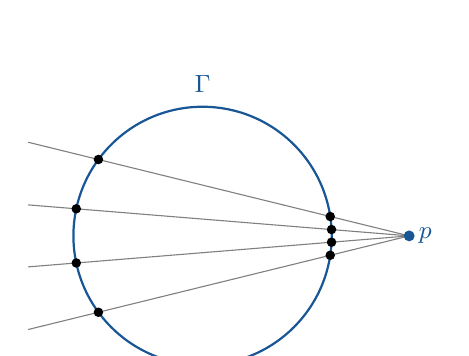
\begin{tikzpicture}[scale=0.82,every node/.style={font=\small}]
  \coordinate (p) at (3.2,0);
  \path[name path=gamma] (0,0) circle (2);
  \draw[thick,linkblue] (0,0) circle (2);
  \foreach \y in {-1.45,-0.48,0.48,1.45}{
    \path[name path=secant] (p)--(-2.7,\y);
    \path[name intersections={of=gamma and secant,name=z}];
    \draw[gray] (p)--(-2.7,\y);
    \fill (z-1) circle (2.1pt);
    \fill (z-2) circle (2.1pt);
  }
  \fill[linkblue] (p) circle (2.4pt) node[right] {$p$};
  \node[linkblue] at (0,2.35) {$\Gamma$};
\end{tikzpicture}
\caption{基准构造（图示取 $n=9$）。经过 $p$ 的四条割线把 $\Gamma$ 上的
八个点配成四对；这四个与 $p$ 共线的点对不产生经过 $p$ 的圆。}
\label{fig:benchmark}
\end{figure}

Elliott 在 1967 年系统研究了这一问题~\cite{elliott}。他的 Theorem~1 证明：任一含 $n>3$
个点的合格点集至少确定
\[
\frac{2n(n-1)}{63}
\]
个恰含三个给定点的圆；这类圆通常称为\emph{普通圆}。他的 Theorem~2 声称
当 $n>393$ 时总圆数至少为 $\binom{n-1}{2}$
~\cite[Theorems~1--2]{elliott}。Purdy--Smith 指出，该结论遗漏了图
~\ref{fig:benchmark} 中与圆外点共线的点对所造成的减项；他们说明 Elliott
的论证可在不改变阈值的前提下修正为 $n\ge394$ 时 $c(n)\ge F(n)$。结合
式~\eqref{eq:F}，这就得到该范围内的 $c(n)=F(n)$
~\cite[\S2.1]{purdy-smith}。

B\'alintov\'a--B\'alint 的 Theorem~2.4 对所有 $n\ge6$ 给出一般的总圆数
二次下界
\[
c(P)\ge \frac{15n(n-1)+1678}{266},
\]
其证明使用 Theorem~2.1 的指定点普通圆下界与 Lemma~6.1 的六点起始情形
~\cite[Theorem 2.1, Theorem 2.4 and Lemma 6.1]{balintova}。另一条相关但不同
的研究线只计普通圆。Zhang 的 Theorem~4.1 证明指定
外点 $q$ 后至少有 $m/6$ 条不经过 $q$ 的普通线，并由反演和双计数得到
Theorem~4.2 的普通圆下界 $\frac19\binom n2$~\cite[Theorems 4.1--4.2]{zhang}。
Lin 等人的 Theorem~1.1(i) 后来确定了充分大 $n$ 时普通圆数的精确最小值
~\cite[Theorem 1.1(i)]{lin-et-al}。这些结果提供强有力的普通圆工具，但它们
并不直接回答本文的总圆数极值：一个高重圆在本文只计一次，却包含许多三元组。

\begin{theorem}\label{thm:main}
对所有 $n\ge4$，均有 $c(n)=F(n)$，仅有三个例外：
\[
c(6)=8=F(6)-1,\qquad c(7)=11=F(7)-2,\qquad
c(8)=17=F(8)-2.
\]
\end{theorem}

Elliott 在 Theorem~2 后记录了 Segre 的观察：立方体的一个平面投影给出
八点反例~\cite[p.~182, discussion following Theorem~2]{elliott}，该构造确定
18 个圆。本文进一步证明最小的例外阶数已经出现在 $n=6$，并把八点反例改进为
$c(P)=17$ 的构造。各例外情形的具体构造见图~\ref{fig:c6}--\ref{fig:c8}。

令 $c_{\mathrm{nc}}(n)$ 表示在所有无三点共线的合格 $n$ 点集中 $c(P)$ 的最小值。
附加这一条件后，答案只在一个阶数发生变化。

\begin{corollary}\label{thm:no-three}
对每个 $n\ge4$，
\[
c_{\mathrm{nc}}(n)=1+\binom{n-1}{2},
\]
唯一例外是 $c_{\mathrm{nc}}(8)=20$。
\end{corollary}

Purdy--Smith 对 Elliott 论证的修正已经解决所有 $n\ge394$ 的情形，因而原则上把
未解决部分化为有限问题~\cite[\S2.1]{purdy-smith}。但实际剩余的关联结构数量巨大、
形态不规则，既无法用小规模直接搜索处理，也不适合用一种简单计算统一验证。本文的
证明不依赖上述大 $n$ 阈值：它直接适用于所有 $n\ge15$，而不只是补齐
$15\le n\le393$；本文还完整解决了无三点共线的加强版本。对原问题的 $n\le14$
情形，则先用数学约束大幅压缩可能的关联数据，再进行精确计算验证。

本项目由作者与人工智能系统分阶段协同完成。作者首先使用中国科学技术大学
JiuChong 团队开发的 AI 辅助数学研究系统 Eureka，得到所有 $n\ge16$ 情形的
数值结果。随后对这些计算的分析表明，$n\ge92$ 部分已经主要由若干不等式控制，
因而几乎可以完全提炼为数学论证；该阶段得到的早期证明收录于
附录~\ref{app:early92}。以此为起点，作者借助 OpenAI Codex 继续加强估计，最终
得到适用于所有 $n\ge15$ 的证明。Codex 还用于完成全部剩余小阶情形的精确验证及
例外构造搜索。论文中的数学证明已被转写为 Lean~4 代码，并在 Mathlib 环境中通过
检查。形式化文件和精确计算文件收录于配套的 GitHub 仓库
\url{https://github.com/LyonWang00/Erdos-problem/tree/main/Erdos506}。

\section{记号与基本工具}

以下固定一个满足定义条件的 $n$ 点集 $P$。令 $K$ 为一条直线或一个圆所能
包含的 $P$ 中点数的最大值，并置 $r=n-K$。达到该最大值的直线或圆分别称为
\emph{最大直线}或\emph{最大圆}。
把至少包含三个点的极大共线子集、极大共圆子集分别称为\emph{直线块}、
\emph{圆块}；无需区分二者时，统称为\emph{块}。

当点标为 $p_0,p_1,\ldots$ 时，下标串表示相应的点子集；例如 $0256$ 表示
$\{p_0,p_2,p_5,p_6\}$。在关联表中，周围文字会说明该子集是共线还是共圆。
这一约定只用于缩短有限列表；若所列点中没有三个非共线点，则下标串本身并不表示一个圆。

为严格表述例外构造的分类，还需区分两种关联类型。称欧氏直线或欧氏圆为
\emph{广义圆}；等价地，它们是黎曼球面
$\widehat{\mathbb C}=\mathbb C\cup\{\infty\}$ 上的圆。记
$\mathcal B_L(P),\mathcal B_C(P)$ 分别为 $P$ 的直线块族与圆块族。

\begin{definition}[关联同构与反演等价]
设 $P,P'$ 是点数相同的有限标号点集。
\begin{enumerate}[label=\textup{(\roman*)}]
\item 若双射 $\sigma:P\to P'$ 满足
\[
 \sigma\bigl(\mathcal B_L(P)\bigr)=\mathcal B_L(P'),\qquad
 \sigma\bigl(\mathcal B_C(P)\bigr)=\mathcal B_C(P'),
\]
则称其为\emph{直线--圆关联同构}。换言之，这种同构不仅保持点与块之间的从属
关系、块的极大性及块的大小，还分别保持直线块族和圆块族。相应的同构类称为
$P$ 的\emph{直线--圆关联类型}。
\item 在集合系 $\mathcal B_L(P)\cup\mathcal B_C(P)$ 中忘记每个块原来是直线还是
圆，所得集合系称为 $P$ 的\emph{广义圆关联结构}；两个这样的集合系之间的同构称为
\emph{广义圆关联同构}，相应的同构类称为\emph{广义圆关联类型}。
\item 把平面等同于复平面。若经过点重标号后，存在
\[
 z\longmapsto\frac{\alpha z+\beta}{\gamma z+\delta},\qquad
 \alpha\delta-\beta\gamma\ne0,
\]
把 $P$ 映到 $P'$，且 $P$ 中没有点被映到 $\infty$，则称二者 \emph{Möbius
等价}。若还允许在上式中以 $\overline z$ 代替 $z$，则称为\emph{扩展 Möbius
等价}；新增的映射即 anti-Möbius 变换。
\end{enumerate}
\end{definition}

Möbius 与 anti-Möbius 变换保持广义圆，故上述几何等价必然诱导广义圆关联同构；
反之一般不成立。还应注意，$c(P)$ 本身并非 Möbius 不变量：经过变换极点的广义圆
会变成欧氏直线，而直线在 $c(P)$ 中不计数。这正是下文既要保留直线--圆类别，
又要考察忘记该类别后的广义圆关联结构的原因。

\subsection{最大共线或共圆子集的直接计数}

\begin{lemma}\label{lem:largest}
若存在一条含 $K$ 个 $P$ 中点的最大直线，则
\begin{equation}\label{eq:DL}
c(P)\ge D_L(n,r):=r\binom K2-\binom r2\left\lfloor\frac K2\right\rfloor.
\end{equation}
若存在一个含 $K$ 个 $P$ 中点的最大圆，则
\begin{equation}\label{eq:DC}
c(P)\ge D_C(n,r):=1+r\left(\binom K2-\left\lfloor\frac K2\right\rfloor\right)
-\binom r2\left\lfloor\frac K2\right\rfloor.
\end{equation}
\end{lemma}

\begin{proof}
固定最大直线或最大圆之外的一点 $q$。在最大直线情形，$q$ 与直线上的任意
点对确定一个圆；固定 $q$ 时这些圆两两不同。在最大圆情形，至多
$\lfloor K/2\rfloor$ 个圆上点对与 $q$ 共线，其余点对各给出一个新圆，另计
该最大圆本身。固定两个外点 $q,q'$。同时出现在两份计数中的每个圆都经过
$q,q'$，并在所选最大直线或最大圆上截出一个二点集。两个不同重复圆所对应的
二点集互不相交；否则两圆还会共享第三点，因而必须重合。故每对 $q,q'$ 的
公共圆至多有 $\lfloor K/2\rfloor$ 个。对这些圆的集合使用第一条
Bonferroni 不等式（集合大小之和减去两两交集大小之和），即得两式；一个圆
同时出现在三份以上计数中不会破坏这一方向的下界。
\end{proof}

\subsection{逐点反演与重数恒等式}

固定 $x\in P$，以 $x$ 为中心反演 $P\setminus\{x\}$，得到 $q=n-1$ 个
非共线点的配置 $Q_x$。事实上，若 $Q_x$ 共线，则其逆像是一条经过 $x$ 的
直线或一个经过 $x$ 的圆，从而 $P$ 全共线或全共圆。令 $t_i(x)$ 为
$Q_x$ 中恰含 $i$ 点的连接线数；令
$b_i(x)$ 为其中经过原几何点 $x$ 的线数，并置
\[
u_i(x)=t_i(x)-b_i(x).
\]
经过反演中心 $x$ 的连接线对应原配置中的直线；不经过 $x$ 的 $i$ 点连接线对应一个
恰含 $i+1$ 个原点、并经过 $x$ 的圆。于是有以下精确恒等式。

\begin{lemma}\label{lem:identities}
对每个 $x\in P$，
\begin{equation}\label{eq:pairs}
\sum_{i=2}^{K-1}\binom i2t_i(x)=\binom{n-1}{2}
\end{equation}
以及
\begin{equation}\label{eq:center-cap}
\sum_{i=2}^{K-1}i b_i(x)\le n-1
\end{equation}
对每个整数 $s\ge2$，还有
\begin{equation}\label{eq:rounded-centre}
\sum_{i\ge s}b_i(x)\le
\left\lfloor\frac{n-1}{s}\right\rfloor.
\end{equation}
若 $\ell_k,c_k$ 分别是 $k$ 点直线、$k$ 点圆的数目，则
\begin{equation}\label{eq:circleexact}
c(P)=\sum_{x\in P}\sum_{i=2}^{K-1}\frac{u_i(x)}{i+1}
\end{equation}
此外，
\begin{equation}\label{eq:incidence}
\sum_xb_i(x)=(i+1)\ell_{i+1},\qquad
\sum_xu_i(x)=(i+1)c_{i+1}
\end{equation}
以及
\begin{equation}\label{eq:triples}
\binom n3=\sum_{k\ge3}\binom k3(\ell_k+c_k)
\end{equation}
特别地，$\sum_xt_i(x)$ 被 $i+1$ 整除。
\end{lemma}

\begin{proof}
式~\eqref{eq:pairs} 按连接线分拆 $Q_x$ 的点对。经过 $x$ 的不同连接线所含的
$Q_x$ 中点互不相交，给出~\eqref{eq:center-cap}。式~\eqref{eq:rounded-centre}
左端所计的每条线至少含有 $s$ 个这样的像点，且不同线所含像点集合互不相交；
又因线数为整数，
故取整即得该式。一个 $k$ 点圆在它的每个点处反演为一条不经过中心的
$(k-1)$ 点线，故在~\eqref{eq:circleexact} 的总和中
恰出现 $k$ 次；直线同理给出~\eqref{eq:incidence}。最后，每个非共线三元组
恰在一个圆上，每个共线三元组恰在一条直线上，得到~\eqref{eq:triples}。
\end{proof}

\subsection{线排列不等式与相交限制}

Elliott 的式~(4)是
\begin{equation}\label{eq:melchior}
t_2(x)\ge3+\sum_{i\ge4}(i-3)t_i(x),
\end{equation}
它来自实射影线排列的 Euler 关系~\cite[Eq.~(4)]{elliott}。当最高三种交点
重数消失时，Hirzebruch 的式~(9)给出
\begin{equation}\label{eq:hirz}
4t_2(x)+3t_3(x)\ge4(n-1)+4\sum_{i\ge5}(2i-9)t_i(x).
\end{equation}
其原始假设是 $t_q=t_{q-1}=t_{q-2}=0$，本文每次使用前都由当前 $K$ 的
上界核验该假设~\cite[\S6, Eq.~(9)]{hirzebruch}。在相应的最大重数假设下，
Bojanowski 不等式可写为
\begin{equation}\label{eq:bojanowski}
4t_2(x)+3t_3(x)\ge4q+\sum_{i\ge5}i(i-4)t_i(x),
\qquad q=n-1,
\end{equation}
其适用条件是不存在含至少 $2q/3$ 个像点的连接线；这正是 Pokora
Theorem~2.1 的点配置对偶形式~\cite[Theorem~2.1]{pokora}。

\begin{lemma}[连接线总数的取整下界]\label{lem:rounded-lines}
在式~\eqref{eq:melchior} 与~\eqref{eq:bojanowski} 适用时，
\begin{equation}\label{eq:rounded-lines}
 \sum_{i\ge2}t_i(x)\ge
 \left\lceil\frac{q^2+3q+9}{9}\right\rceil .
\end{equation}
\end{lemma}

\begin{proof}
把点对恒等式~\eqref{eq:pairs}、Melchior 不等式~\eqref{eq:melchior} 与
Bojanowski 不等式~\eqref{eq:bojanowski} 分别乘以 $2/9,1/3,1/9$ 后相加。
对 $i\ge5$，$t_i$ 的系数为
\[
 \frac{2}{9}\binom i2-\frac{i-3}{3}-\frac{i(i-4)}9=1;
\]
$i=2,3,4$ 时直接代入同样得到系数 $1$。右端为
$(q^2+3q+9)/9$，左端为整数，故可向上取整。
\end{proof}

把 Zhang 的 Theorem~4.1 应用于非共线像点集 $Q_x$ 及不属于该像点集的
外点 $x$~\cite[Theorem~4.1]{zhang}，得到
\begin{equation}\label{eq:zhang}
u_2(x)\ge\left\lceil\frac{n-1}{6}\right\rceil,
\end{equation}
而 Csima--Sawyer 的主定理（$n>7$）给出
$t_2(x)\ge\lceil6(n-1)/13\rceil$~\cite[Theorem on pp.~187--188]{csima-sawyer}。

将 $Q_x$ 中至少含四点的连接线按所含点数非增排列为
$L_1,L_2,\ldots$，则任意前 $j$ 条满足
\begin{equation}\label{eq:prefix}
\sum_{a=1}^j|L_a|-\binom j2\le n-1,
\end{equation}
因为两条不同直线至多有一个公共点。固定一条含 $a$ 点的连接线后，线内外的
$a(n-1-a)$ 个点对必须分别属于其他连接线；固定两条分别含 $a,b$ 点的连接线
后，去掉两线可能的交点，仍有 $(a-1)(b-1)$ 个跨线点对。因此得到必要条件
\begin{equation}\label{eq:oneline}
\sum_i(i-1)t_i-(a-1)\ge a(n-1-a)
\end{equation}
以及
\begin{equation}\label{eq:twoline}
\sum_it_i-2\ge(a-1)(b-1)
\end{equation}
式~\eqref{eq:prefix}--\eqref{eq:twoline} 虽不是几何可实现性的充分条件，却能
在坐标问题出现之前排除大量不可能的整数重数向量。

下面给出一种同时利用多个反演中心的方法。若 $\mathcal C_k$ 是所讨论的
$k$ 点圆的集合，记 $g_k=|\mathcal C_k|$，并令 $d_k(x)$ 为 $\mathcal C_k$
中经过 $x$ 的圆数。两个不同圆至多有两个公共点，因而
\begin{equation}\label{eq:samesupport}
\sum_x\binom{d_k(x)}2\le2\binom{g_k}{2}
\end{equation}
并且当 $k\ne m$ 时，
\begin{equation}\label{eq:crosssupport}
\sum_xd_k(x)d_m(x)\le2g_kg_m
\end{equation}
这两式把不同反演中心处的局部下界联系起来，是处理 $n\le33$、尤其是
$n=15$ 时的关键补充。

\begin{lemma}[圆族关联度的二阶矩估计]\label{lem:support-moment}
设 $\mathcal C_k,\mathcal C_m$ 分别是 $g_k,g_m$ 个 $k$ 点圆、$m$ 点圆组成的圆族，
$d_k(x),d_m(x)$ 分别表示两族中经过 $x$ 的圆数。若某个局部计数 $\Phi_x$ 满足
\[
\Phi_x\ge \alpha+\beta d_k(x)+\beta'd_m(x)
-\gamma\binom{d_k(x)}2-\gamma'\binom{d_m(x)}2
-\eta d_k(x)d_m(x),
\]
其中 $\gamma,\gamma',\eta\ge0$，则
\begin{align}
\sum_{x\in P}\Phi_x\ge{}&n\alpha+\beta k g_k+\beta'mg_m
-2\gamma\binom{g_k}{2}-2\gamma'\binom{g_m}{2}
-2\eta g_kg_m. \label{eq:support-moment}
\end{align}
\end{lemma}

\begin{proof}
双计数给出 $\sum_xd_k(x)=kg_k$ 及 $\sum_xd_m(x)=mg_m$。对局部不等式
求和，再将~\eqref{eq:samesupport}--\eqref{eq:crosssupport} 代入所有非正的
二次项，即得~\eqref{eq:support-moment}。
\end{proof}

这个引理把所有中心处关联度分布的枚举替换成一个有限的不等式拟合问题：
只需为有限表中的局部最小值寻找形如上式的二次下界。
单圆族情形令 $d_m=0$即可。多圆族情形的混合项则直接使用
两族圆两两至多交于两点。这个简单的二阶矩估计将在后文多次使用。

\section{\texorpdfstring{$n\ge17$}{n>=17} 的数学证明}

令 \(q=n-1\)。回忆 \(K\) 是原点集中一条直线或一个圆所含点数的最大值，
故每个反演像 \(Q_x\) 中的连接线至多含 \(K-1\) 个像点。记
\[
\Phi_x=\sum_{i=2}^{K-1}\frac{t_i(x)-b_i(x)}{i+1}.
\]
由式~\eqref{eq:circleexact}，\(c(P)=\sum_x\Phi_x\)。

\begin{lemma}\label{lem:bojanowski-local}
若
\begin{equation}\label{eq:bojanowski-range}
 3(K-1)<2(n-1),
\end{equation}
则对每个 \(x\in P\)，
\begin{equation}\label{eq:bojanowski-local}
\Phi_x\ge
 \frac{K+1}{18K}\binom q2+\frac{K+1}{2K}
 +\frac{K-2}{9K}q-\frac13\left\lfloor\frac q2\right\rfloor.
\end{equation}
\end{lemma}

\begin{proof}
条件~\eqref{eq:bojanowski-range} 正是使用 Bojanowski 不等式
\[
4t_2+3t_3\ge4q+\sum_{i\ge5}i(i-4)t_i
\]
所需的最大重数条件~\cite[Theorem~2.1]{pokora}。分别以
\[
 \alpha=\frac{K+1}{18K},\qquad
 \beta=\frac{K+1}{6K},\qquad
 \gamma=\frac{K-2}{36K}
\]
乘点对恒等式、Melchior 不等式及上述 Bojanowski 不等式后相加。
所得 \(t_i\) 的系数不超过 \(1/(i+1)\)。在 \(i=2,3\) 时系数相等；
在 \(i=4\) 及 \(5\le i\le K-1\) 时，两者之差分别为
\[
 \frac{K-5}{30K},\qquad
 \frac{(i-3)(i-2)(K-i-1)}{12K(i+1)},
\]
均非负。（当 \(K=3,4\) 时不存在 \(i=4\) 项。）因此
\[
 \sum_i\frac{t_i(x)}{i+1}\ge
 \alpha\binom q2+3\beta+4q\gamma.
\]
被 \(b_i(x)\) 计数的连接线都经过反演中心，且它们所含的像点集合两两不交，故
\[
 \sum_i b_i(x)\le\left\lfloor\frac q2\right\rfloor,\qquad
 \sum_i\frac{b_i(x)}{i+1}\le
 \frac13\left\lfloor\frac q2\right\rfloor.
\]
这就证明了式~\eqref{eq:bojanowski-local}。
\end{proof}

\begin{theorem}\label{thm:nge17}
若 \(n\ge17\)，则每个合格 \(n\) 点集 \(P\) 均满足 \(c(P)\ge F(n)\)。
\end{theorem}

\begin{proof}
先设式~\eqref{eq:bojanowski-range} 成立。对全部 \(n\) 个反演中心求和，
再减去 \(F(n)-1\)。当 \(n\) 为偶数时，式~\eqref{eq:bojanowski-local}
给出的余量为
\begin{equation}\label{eq:even-margin}
 \frac{Kn^3-23Kn^2+100Kn-72K+n^3-11n^2+28n}{36K};
\end{equation}
当 \(n\) 为奇数时，余量为
\begin{equation}\label{eq:odd-margin}
 \frac{Kn^3-23Kn^2+94Kn-54K+n^3-11n^2+28n}{36K}.
\end{equation}
两式关于 \(K\) 均单调递减，因为导数都是
\[
 -\frac{n(n-7)(n-4)}{36K^2}.
\]
式~\eqref{eq:bojanowski-range} 给出 \(K\le(2n+1)/3\)。在这个连续
右端点处，式~\eqref{eq:even-margin} 与式~\eqref{eq:odd-margin}
分别化为
\[
 \frac{n^4-21n^3+72n^2+20n-36}{18(2n+1)},\qquad
 \frac{n^4-21n^3+66n^2+35n-27}{18(2n+1)}.
\]
对偶数 \(n=18+2u\) 和奇数 \(n=19+2u\)，两个分子分别为
\[
\begin{split}
16u^4+408u^3+3528u^2+11056u+6156,\\
16u^4+440u^3+4140u^2+14472u+10746,
\end{split}
\]
故在 \(u\ge0\) 时均为正。对 \(n=17\)，整数性给出 \(K\le11\)，
式~\eqref{eq:odd-margin} 的最小值为 \(10/33\)。因此
\(c(P)>F(n)-1\)，再由整数性得到 \(c(P)\ge F(n)\)。

下面设 \(3(K-1)\ge2(n-1)\)。因 \(n\ge17\)，此时必有 \(3K\ge n+12\)。
令 \(r=n-K\)。利用 \(\lfloor K/2\rfloor\le K/2\)，
引理~\ref{lem:largest} 中最大子集为直线和圆的两个下界分别给出
\[
 D_L(n,r)\ge \frac{rK(3K-n-1)}4
     =B(n,K)+\frac{rK}{2}-1\ge B(n,K)
\]
与
\[
 D_C(n,r)\ge1+\frac{rK(3K-n-3)}4=B(n,K),
\]
其中
\begin{equation}\label{eq:coarse}
 B(n,K):=1+\frac{(n-K)K(3K-n-3)}4.
\end{equation}
在实区间 \((n+12)/3\le K\le n-2\) 上，\(B\) 的导数是开口向下的
二次式；它在左端点的值为
\[
 \frac{2n^2+21n-360}{12}>0.
\]
开口向下的二次式从左端的正值出发，在该区间至多从正变负一次。因此
\(B\) 或始终递增，或先增后减，不会在区间内部取得最小值。利用
\(F(n)\le(n^2-4n+6)/2\)，两个端点处的余量分别为
\[
 5n-38,\qquad \frac{(n-7)(n-2)}2,
\]
均为正。当 \(K=n-1\) 时，式~\eqref{eq:DC} 的精确最大圆下界恰为
\(F(n)\)，而最大直线下界还多出 \(\lfloor K/2\rfloor-1\)。
补充分支也由此闭合。
\end{proof}

随附的代数核验器用精确符号运算展开上述全部系数差与奇偶多项式；
它不枚举 \(n\)、\(K\) 或任何线重数型。

\section{\texorpdfstring{$n=16$}{n=16} 的证明}
\label{sec:n16}

局部下界~\eqref{eq:bojanowski-local} 在 \(n=16\) 时仍然有效。
对 \(K=3,4,5,6\)，逐点下界及总和超过 \(98\) 的余量为
\[
\begin{array}{c|cccc}
K&3&4&5&6\\ \hline
 \Phi_x&20/3&77/12&94/15&37/6\\
 16\Phi_x-98&26/3&14/3&34/15&2/3.
\end{array}
\]
对 \(K=9,\ldots,15\)，引理~\ref{lem:largest} 中直线界与圆界的较小者依次为
\[
141,166,201,205,199,162,99,
\]
均不小于 \(F(16)=99\)。下面用数学方法闭合 \(K=7,8\)，不再使用有限验证。

先设 \(K=7\)，令 \(d_x=t_6(x)-b_6(x)\)，即经过 \(x\) 的七点圆数。
省略中心下标，并记
\[
\begin{aligned}
 T&=\sum_{i=2}^6\binom i2t_i,&
 M&=t_2-\sum_{i=4}^6(i-3)t_i,\\
 B&=4t_2+3t_3-\sum_{i=5}^6i(i-4)t_i,&
 S&=\sum_{i=2}^6b_i.
\end{aligned}
\]
点对恒等式、Melchior、Bojanowski 以及经过反演中心的不同连接线所含像点
集合互不相交，分别给出
\[
 T=105,\qquad M\ge3,\qquad B\ge60,\qquad S\le7.
\]
逐项比较系数得到恒等式
\begin{equation}\label{eq:n16-k7-identity}
\begin{split}
 \Phi_x+\frac{d_x}{42}
={}&\frac7{108}T+\frac7{36}M+\frac1{54}B-\frac13S+R_7,\\
 R_7={}&\frac{t_4}{180}+\frac{b_3}{12}+\frac{2b_4}{15}
          +\frac{b_5}{6}+\frac{b_6}{6}\ge0.
\end{split}
\end{equation}
因此
\begin{equation}\label{eq:n16-k7-local}
 \Phi_x+\frac{d_x}{42}\ge\frac{37}{6}.
\end{equation}

设七点圆共有 \(g\) 个。四个这样的圆不能经过同一点，否则反演后四条
六点线之并至少含 \(4\cdot6-\binom42=18>15\) 个像点。因此 \(d_x\le3\)，且
\[
 \sum_xd_x=7g,\qquad
 \sum_x\binom{d_x}{2}\le2\binom g2=g(g-1).
\]
当 \(g=5,6\) 时，对 \(0\le d\le3\) 使用
\(\binom d2\ge2d-3\)，所得下界 \(14g-48=22,36\) 分别超过上界
\(20,30\)。当 \(g\ge7\) 时，\(7g=\sum_xd_x\le16\cdot3\) 不成立。
对 \(g\le3\)，式~\eqref{eq:n16-k7-local} 求和给出
\[
 c(P)\ge\frac{296}{3}-\frac g6
       =98+\frac{4-g}{6}>98.
\]

只需再排除 \(g=4\) 的等号。若没有 \(d_x=1\) 的点，则
\(d_x\in\{0,2,3\}\) 且 \(\binom{d_x}{2}\ge d_x/2\)，从而二阶关联矩至少
为 \(14>12\)。故可选 \(d_x=1\) 的点。若 \(c(P)=98\)，则
式~\eqref{eq:n16-k7-identity} 中所有正余项和所用不等式都必须取等。
Melchior、Bojanowski 及点对恒等式于是唯一确定
\[
 (t_2,t_3,t_4,t_5,t_6)=(14,12,0,4,1),\qquad
 (b_2,b_3,b_4,b_5,b_6)=(7,0,0,0,0).
\]
其中四条五点线和一条六点线之并至少含
\(4\cdot5+6-\binom52=16\) 个像点，矛盾。故 \(K=7\) 的情形得证。

下面设 \(K=8\)。在选定最大八点直线或圆上的任一点反演，其余七点均落在
一条七点像线上。记
\[
 O=t_2-b_2,\qquad I=\sum_{i=2}^7(i-1)t_i,\qquad
 S=\sum_{i=2}^7b_i,
\]
并把 \(T,M\) 的求和上限改为 \(7\)。普通线下界、式~\eqref{eq:center-cap}
以及该七点像线
的关联计数给出
\[
 O\ge3,\qquad S\le7,\qquad I\ge6+7(15-7)=62.
\]
另一条系数恒等式为
\begin{equation}\label{eq:n16-k8-identity}
\begin{split}
 \Phi_x={}&\frac1{80}T+\frac{31}{160}M+\frac1{48}O
        -\frac5{16}S+\frac{17}{160}I+R_8,\\
 R_8={}&\frac{t_5}{240}+\frac{3t_6}{560}+\frac{b_3}{16}
 +\frac{9b_4}{80}+\frac{7b_5}{48}+\frac{19b_6}{112}
 +\frac{3b_7}{16}\ge0.
\end{split}
\end{equation}
因此最大块上的八个中心均满足 \(\Phi_x\ge1017/160\)，其余八个中心由
式~\eqref{eq:bojanowski-local} 满足 \(\Phi_x\ge145/24\)。于是
\[
 8\cdot\frac{1017}{160}+8\cdot\frac{145}{24}-98=\frac{71}{60}>0.
\]
故 $c(16)\ge99=F(16)$。随附核验器只用精确有理数展开
式~\eqref{eq:n16-k7-identity} 与式~\eqref{eq:n16-k8-identity}，并核对上述
等号型和关联矩计算；它不含优化模型或重数向量枚举。

\section{十五点情形}\label{sec:n15}

本节证明 $c(15)=85$。令 $K$ 为合格点集 $P$ 中一条直线或一个圆所含点数的
最大值。若 $K\ge8$，引理~\ref{lem:largest} 给出 $c(P)\ge85$，故以下设
$K\le7$。

固定 $x\in P$，以 $x$ 为中心反演其余十四点，再将所得点集对偶化，得到十四条
实射影直线的排列。记其 $r$ 重交点数为 $t_r(x)$，并定义
\[
 \delta_x=t_2(x)-3-\sum_{r=4}^{6}(r-3)t_r(x).
\]
Melchior 关系表明，$\delta_x$ 等于各面边数超过三的总量，因而
$\delta_x\ge0$。

直线数为偶数还排除了 $\delta_x=1$。事实上，十四个齐次线性方程之积的符号
在射影平面上良定义，从而给出面的二染色。若
$E=\sum_r r t_r(x)$ 为边数，$F_+,F_-$ 为两种颜色的面数，则
\[
 \varepsilon_+=E-3F_+,
 \qquad \varepsilon_-=E-3F_-
\]
均为非负整数，模 $3$ 同余，且
$\delta_x=\varepsilon_++\varepsilon_-$。故二者之和不可能为一。

定义与中心 $x$ 相关的整数
\begin{equation}\label{eq:n15-residual}
 R_x=136t_2(x)+93t_3(x)+60t_4(x)+30t_5(x)-2902.
\end{equation}
先证 $R_x\ge0$。点对恒等式与 $\delta_x$ 的定义给出
\[
 3t_3+7t_4+12t_5+18t_6=88-\delta_x.
\]
最大交点重数不超过六，故 Bojanowski 不等式的前提满足，并有
\[
 4t_2+3t_3-5t_5-12t_6\ge56.
\]
消去 $t_2,t_3$，得到
\begin{equation}\label{eq:n15-rich-bound}
 3t_4+9t_5+18t_6\le44+3\delta_x
\end{equation}
及
\begin{equation}\label{eq:n15-residual-delta}
 R_x=234+105\delta_x-21t_4-70t_5-150t_6.
\end{equation}
若 $\delta_x\ge2$，则由式~\eqref{eq:n15-rich-bound}
\[
21t_4+70t_5+150t_6
 \le25(t_4+3t_5+6t_6)
 \le\frac{25}{3}(44+3\delta_x),
\]
所以 $R_x\ge(240\delta_x-398)/3$。由于 $R_x$ 是整数，遂有 $R_x\ge28$。

只剩 $\delta_x=0$，此时线排列是单纯的。Cuntz 对至多二十七条线的完整分类
~\cite[Theorem~1.1 及不变量表中十四线的条目，p.~696]{cuntz} 表明，排除含
七重交点的类型及近铅笔排列后，$(t_2,t_3,t_4,t_5,t_6)$ 只有
\[
 (11,12,4,2,0),\qquad(9,16,4,1,0),\qquad(10,14,4,0,1).
\]
相应的 $R_x$ 依次为 $10,80,0$。因此
\begin{equation}\label{eq:n15-residual-gap}
 R_x\ge0,
 \qquad R_x>0\Longrightarrow R_x=10\ \hbox{或}\ R_x\ge28.
\end{equation}

记 $\ell_k,c_k$ 分别为极大的 $k$ 点直线数和 $k$ 点圆数，并令
$C=\sum_{k=3}^{7}c_k=c(P)$。使用精确恒等式
\[
 \ell_2+\sum_{k=3}^{7}\binom{k}{2}\ell_k=\binom{15}{2},
 \qquad
 \sum_{k=3}^{7}\binom{k}{3}(\ell_k+c_k)=\binom{15}{3},
\]
以及
\[
 \sum_{x\in P}t_{k-1}(x)=k(\ell_k+c_k)\qquad(3\le k\le7).
\]
Csima--Sawyer 定理给出
$\ell_2\ge\lceil90/13\rceil=7$~\cite[pp.~187--188 的主定理]{csima-sawyer}。
把上述恒等式直接代入，得到
\begin{align}\label{eq:n15-global-identity}
420C-35270={}&140(\ell_2-7)+420\ell_4+980\ell_5
 +1680\ell_6+2520\ell_7+\sum_{x\in P}R_x.
\end{align}
右端各项非负，故 $C\ge84$。

若 $C=84$，式~\eqref{eq:n15-global-identity} 左端为 $10$。于是
$\ell_2=7$、$\ell_4=\cdots=\ell_7=0$ 且 $\sum_xR_x=10$。
由式~\eqref{eq:n15-residual-gap}，恰有一个中心的局部重数向量为
$(11,12,4,2,0)$，其余十四个中心均为 $(10,14,4,0,1)$。因此
\[
 \sum_{x\in P}t_2(x)=11+14\cdot10=151.
\]
但 $k=3$ 的局部关联恒等式说明同一个和等于 $3(\ell_3+c_3)$，矛盾。
故 $C\ge85$。式~\eqref{eq:F} 的构造给出 $F(15)=85$，从而
$c(15)=85$。

\begin{remark}
本节没有选择直线或圆所含的带标号点子集，也没有枚举几何轨道。唯一的有限输入
是 Cuntz 的完整十四线表中
列出的三个重数向量；其余步骤均为整数恒等式和不等式。
\end{remark}

\section{\texorpdfstring{$9\le n\le14$}{9<=n<=14} 的情形}
\label{sec:small-uniform}

本节把仅需全局整数数据即可处理的两个较大情形，与仍需精确有限验证的四个较小情形分开叙述。整个证明不读取历史搜索树，也不使用预存的轨道表。

对 $k\ge3$，以 $\ell_k$ 和 $c_k$ 分别表示极大 $k$ 点直线与极大
$k$ 点圆的数目，并令 $m_k=\ell_k+c_k$。每个点对属于唯一的极大直线；每个三点组
或者属于其极大直线，或者属于唯一的外接圆。因此
\begin{align}
 \ell_2+\sum_{k\ge3}\binom{k}{2}\ell_k&=\binom n2,
 \label{eq:small-line-pairs}\\
 \sum_{k\ge3}\binom{k}{3}m_k&=\binom n3,
 \qquad \sum_{k\ge3}c_k=c(P).
 \label{eq:small-triple-partition}
\end{align}
称 $(\ell_3,\ldots,\ell_K;c_3,\ldots,c_K)$ 为一个\emph{全局计数向量}。引理~\ref{lem:largest} 分别排除
$n=9,10,11,12,13,14$ 时大小至少为 $6,7,7,7,7,8$ 的块，故以下各分支只需考虑
$K\le5,6,6,6,6,7$。

计数向量的生成只使用必要条件。由于 $K<n-1$，删除任意一点后所得点集仍满足本问题的条件，对所有删除求和得到
\begin{equation}\label{eq:small-one-delete}
 n c(P)-3c_3\ge n c(n-1).
\end{equation}
在每一点反演后应用 Zhang 的指定外点普通线定理
\cite[Theorem~4.1]{zhang}，得到
\begin{equation}\label{eq:small-z-circle}
 3c_3\ge n\left\lceil\frac{n-1}{6}\right\rceil.
\end{equation}
此外，对计数向量的直线部分使用普通线、Melchior、Hirzebruch--Bojanowski 与 Shnurnikov 不等式，并在必定非共线的子集上求和
\cite[Eq.~(9)]{hirzebruch}\cite[Theorem~2.1]{pokora}\cite[Theorem~3]{shnurnikov}。
若子集包含在一条极大直线中，则不对它使用圆数下界；若子集包含在一个极大圆中，则只要求保留该圆。这是小阶删除平均中必须加入的修正。

还需用到块的交集所给出的下列初等不等式。对 $N\ge1$ 以及
$S=aN+b$（$0\le b<N$），令
\[
 \Phi_N(S)=N\binom a2+ab.
\]
它是满足 $\sum_i x_i=S$ 的非负整数向量中
$\sum_i\binom{x_i}{2}$ 的最小值。任取 $L$ 条极大直线和 $G$ 个极大圆，记它们的总点关联数和总点对关联数为 $I_1,I_2$，则
\begin{align}
 \Phi_n(I_1)&\le \binom L2+2LG+2\binom G2,
 \label{eq:small-block-point}\\
 \Phi_{\binom n2}(I_2)&\le LG+\binom G2.
 \label{eq:small-block-pair}
\end{align}
这是因为两条直线至多交于一点，而其余任意两个不同块至多交于两点。把每一类的
块按大小排列，并对每个初始段应用这两个不等式，即可覆盖所有子族；这一过程不必
决定哪些带标号的点实际落在所选直线或圆上。

\subsection{增广直线不等式}

固定 $x\in P$，以 $x$ 为中心反演，再对其余 $n-1$ 个像点作射影对偶。记所得直线排列中重数为 $j$ 的顶点数为 $t_j(x)$，并令
\[
 \delta_x=t_2(x)-3-\sum_{j\ge4}(j-3)t_j(x).
\]
以 $d_k^L(x)$ 表示经过 $x$ 的极大 $k$ 点直线数。

\begin{lemma}\label{lem:augmented-line}
对每个 $x\in P$，均有
\begin{equation}\label{eq:augmented-line-point}
 \sum_{k\ge3}k d_k^L(x)\le n-1+\delta_x.
\end{equation}
因此
\begin{equation}\label{eq:augmented-line-summed}
 \sum_{k\ge3}k^2\ell_k\le n(n-1)+D,
 \qquad
 D=3m_3-3n-\sum_{k\ge5}k(k-4)m_k.
\end{equation}
\end{lemma}

\begin{proof}
记上述 $n-1$ 条对偶直线的排列为 $\mathcal A_x$，再加入反演中心的对偶直线。经过 $x$ 的一条原 $k$ 点直线，对应于新增直线上的一个旧的 $(k-1)$ 重顶点。设这些旧顶点的重数为 $i_1,\ldots,i_s$。新增直线产生
$(n-1)-\sum_j i_j$ 个新的普通顶点；每把一个旧顶点的重数提高一，Melchior 亏量减少一，这对二重和三重顶点也成立。因此增广排列的亏量为
\[
 \delta_x+(n-1)-\sum_{j=1}^s(i_j+1)
 =\delta_x+(n-1)-\sum_{k\ge3}k d_k^L(x).
\]
增广排列是本质排列，故 Melchior 不等式给出
\eqref{eq:augmented-line-point}。再对 $x$ 求和，并使用
$\sum_xd_k^L(x)=k\ell_k$ 及局部关联恒等式，即得
\eqref{eq:augmented-line-summed}。
\end{proof}

\subsection{十三点与十四点的全局排除}

当 $n=14$ 时，在 $c(P)<F(14)$ 下，前述必要条件的全部整数解共有 8981 个。
不等式~\eqref{eq:augmented-line-summed} 排除其中 8980 个；唯一剩余的计数向量为
\[
 (\ell_3,\ldots,\ell_7;c_3,\ldots,c_7)
 =(20,0,0,0,0;23,44,0,2,3).
\]
其中三个七点圆两两至多交于两点，故其并至少含
$3\cdot7-3\cdot2=15$ 点，矛盾。因此 $c(14)=F(14)$。

当 $n=13$ 时，小于 $F(13)$ 的整数计数向量共有 3962 个。增广直线不等式后剩 137 个，再由
\eqref{eq:small-block-point}--\eqref{eq:small-block-pair} 剩 73 个。以下两条不等式排除全部剩余向量。

在任一点处，局部排列含十二条直线；在当前分支中，其顶点重数不超过五。将其重数向量记为
$(t_2,t_3,t_4,t_5)$，亏量记为 $\delta$。则
\begin{equation}\label{eq:n13-local-two-ineq}
 -2\delta+t_4+3t_5\le6,
 \qquad -\delta+t_5\le1.
\end{equation}
为证明第一式，由点对恒等式及 Bojanowski 不等式有
\begin{align*}
 t_2+3t_3+6t_4+10t_5&=66,\\
 4t_2+3t_3&\ge48+5t_5,
\end{align*}
从而
\[
 H:=3t_2-6t_4-15t_5+18\ge0.
\]
令 $E=2t_2-3t_4-7t_5$。由 $H+3\delta=3(E+3)$ 得
$E\ge-3$；点对恒等式又给出 $E\equiv0\pmod3$。若 $E=-3$，则必有
$H=\delta=0$。Cuntz 对单纯十二线排列的完备分类在排除六重顶点后只留下
$(8,10,3,1)$ 和 $(9,7,6,0)$，而二者均满足 $E=0$
\cite[Theorem~1.1 and the invariant tables]{cuntz}。故 $E\ge0$，这等价于
\eqref{eq:n13-local-two-ineq} 的第一式。

为证明第二式，四个五重顶点对偶为四条五点线，其并至少含
$20-\binom42=14$ 点，故 $t_5\le3$。若 $\delta\ge2$，结论立即成立；若
$\delta=0$，上述 Cuntz 类型均满足 $t_5\le1$。唯一尚可能违反不等式的是
$(\delta,t_5)=(1,3)$。此时点对恒等式与亏量恒等式迫使
$(t_2,t_3,t_4,t_5)=(12,4,2,3)$。但三条五点线与一条四点线的并至少含
$5+5+5+4-\binom42=13$ 点，再次矛盾。第二式得证。

对十三个中心求和，\eqref{eq:n13-local-two-ineq} 化为
\begin{equation}\label{eq:n13-global-two-ineq}
 -2D+5m_5+18m_6\le78,
 \qquad -D+6m_6\le13.
\end{equation}
在最后 73 个计数向量中，71 个违反第一式，其余两个违反第二式。这里仅是把整数计数向量代入
\eqref{eq:n13-global-two-ineq}，没有选择任何带标号点子集。因此 $c(13)=F(13)$。

\subsection{九点至十二点的精确验证}

对 $9\le n\le12$，同一组全局条件与
\eqref{eq:augmented-line-summed} 留下少量非空边界。下面给出统一验证的每一步。固定一点 $x$，以 $a_k(x),u_k(x)$ 分别表示经过 $x$ 的极大
$k$ 点直线和圆的数目，则
\[
 t_{k-1}(x)=a_k(x)+u_k(x),
 \qquad
 \sum_{j\ge2}\binom j2t_j(x)=\binom{n-1}{2}.
\]
这些局部重数向量满足前述公开的直线排列不等式、块交集不等式及
\eqref{eq:augmented-line-point}。第一个整数模型只记录每种局部重数向量出现多少次，并要求
\[
 \sum_xa_k(x)=k\ell_k,\qquad
 \sum_xu_k(x)=kc_k,\qquad
 \sum_x\delta_x=D.
\]

后两个阶段仍不指定带标号的点子集。对块类别 $\alpha$，令 $d_\alpha(x)$ 为包含
点 $x$ 的该类块数，令
$\lambda_\alpha(e)$ 为点对 $e$ 上的度；若块大小为 $k_\alpha$、数目为
$N_\alpha$，则
\begin{align}
 \sum_xd_\alpha(x)&=k_\alpha N_\alpha,&
 \sum_e\lambda_\alpha(e)&=\binom{k_\alpha}{2}N_\alpha,
 \label{eq:small-category-totals}\\
 \sum_\alpha(k_\alpha-2)\lambda_\alpha(e)&=n-2.
 \label{eq:small-pair-profile2}
\end{align}
最后一个恒等式来自：经过 $e$ 的所有极大块在 $e$ 外的部分恰好分割
$P\setminus e$。点数据与点对数据还须满足
\[
\sum_{y\ne x}\lambda_\alpha(\{x,y\})
=(k_\alpha-1)d_\alpha(x).
\]
随后，对任意两个块类别使用精确的交集计数恒等式
\[
 N_2=M_2,\qquad N_1=M_1-2M_2,\qquad N_0=Q-M_1+M_2,
\]
其中 $M_1$ 是所有不同块对交集大小之和，$M_2$ 是这些交集大小的二阶二项式
系数之和，$N_s$ 是恰交于 $s$ 点的不同块对数；模型还精确计数与一个指定块不交的
三点组。所有系数均来自二项式计数，不使用浮点松弛。

最后，以 $x$ 为中心反演会确定一个完整的 $(n-1)$ 点像集计数向量：经过
$x$ 的块变为少一个点的像直线，不经过 $x$ 的块变为像圆。只有当该子向量在下一层
未被排除时，当前局部重数向量才被保留；随后再次平衡全部 $n$ 个点处的数据。递归在
$n=9$ 终止。九点模型在带标号点集的所有子集中选择极大直线与圆，要求每个三点组恰属于一个块、每个点对至多属于一条所选直线，并对每个满足本问题条件的真子集使用已经证明的圆数下界。这个抽象模型比几何实现更宽松，故其不可行足以推出几何不可行。

最终重放的精确数量如下：
\begin{center}
\small
\begin{tabular}{c|rrrrrrr}
\toprule
$n$ & 初始 & 增广求和 & 局部向量 & 点--点对 & 交集计数 & 块对 & 终点\\
\midrule
9  &45   &36  &23  &-- &-- &-- &0\\
10 &180  &150 &55  &26 &21 &12 &1\\
11 &416  &160 &70  &39 &28 &-- &0\\
12 &1354 &211 &169 &55 &44 &-- &0\\
\bottomrule
\end{tabular}
\end{center}
“初始”一列分别由 129、551、1215、4322 个原始计数向量缩减而来。
$n=11,12$ 的终点零由同一个递归器得到；它们分别访问
\[
 (28,72,222)\quad\text{与}\quad(44,322,661,622)
\]
个 $(11,10,9)$ 阶及 $(12,11,10,9)$ 阶计数向量。每个被排除的状态均为精确的
\texttt{INFEASIBLE}，没有 \texttt{UNKNOWN}。

当 $n=10$ 时，递归只留下一个完整计数向量
\[
 (\ell_3,\ell_4,\ell_5,\ell_6;
   c_3,c_4,c_5,c_6;\ell_2)
 =(10,0,0,0;10,20,2,0;15).
\]
递归证书保留的四种局部重数向量均满足 $u_5(x)=1$ 与 $a_3(x)\le3$。两个五点圆共有十个
点关联，故它们恰好把十点分割为 $A,B$。十条三点线共有三十个点关联，故每点均有
$a_3(x)=3$；相应的唯一平衡局部向量还满足 $u_4(x)=8$。每个四点圆因而在 $A,B$ 两侧
各取两点。

把这样的四点圆对应于其在 $A$ 与 $B$ 中的两条弦。两弦的交点位于两个五点圆的
固定根轴上。圆上五点所确定的弦中，不可能有三条在圆外同点：三条两两不共端点的
弦需要六个端点。因此，在根轴同一点相交的两侧弦数都至多为二。二十个四点圆达到
该上界，弦图遂恰为五个互不相交的 $K_{2,2}$。在 $S_5\times S_5$ 作用下，
Petersen 图的六个完美匹配给出两个双陪集轨道。其中一个不存在相容的十条三点线
设计，另一个有两个互补设计，二者属于同一轨道。

对后一个轨道取代表元，十条直线关联给出含非零参数 $a,b,d$ 的完备射影参数化。选取五个圆交点矩阵的三阶子式，得到
\begin{gather*}
 ad+b^2,\quad -ab+ad-b,\quad ab-ad-a-1,\\
 -ad+bd-b-d,\quad b(ab+1).
\end{gather*}
它们必须同时为零。第二、三式相加给出 $a+b+1=0$，而末式及 $b\ne0$ 给出
$ab+1=0$，故 $b^2+b-1=0$。第一式给出
$d=b^2/(b+1)$；这里 $b+1=-a\ne0$。再代入第四式并移去非零因子，得到
\[
 (b-1)(2b+1)=0,
\]
它与 $b^2+b-1$ 互素。被舍弃的参数分支会使两个带标号点重合；形成原始子式时除去的因子只可能是
$a,d,b,ad$，它们均非零。因此最后一个十点计数向量也不可能实现。

结合式~\eqref{eq:F} 的构造，得到
\[
 c(n)=F(n)\qquad(9\le n\le14).
\]

\begin{remark}[有限验证的范围]
本节只有九点终止模型实际选择带标号点的子集。十点至十二点只使用计数向量及
局部重数的递归一致性，十三点与十四点只使用全局不等式。证明不对任意直线排列假设
$\sum_jt_j\ge2r-4$；对含 $q$ 条直线的排列，Elliott 的 Theorem~3 仅在明确满足
$q\ge10$ 且不存在 $(q-1)$ 重顶点时使用。
\end{remark}


\section{\texorpdfstring{$4\le n\le8$}{4<=n<=8} 的有限情形}

下述两个初等事实将在本节反复使用。
\begin{lemma}\label{lem:two-line-geometry}
设实射影平面中的 $A,B,C,D$ 无三点共线，则
$AB\cap CD$、$AC\cap BD$、$AD\cap BC$ 三点不共线。又设一个圆与两条直线
各交于两个给定点。若两直线相交，并以交点为原点在两线上取有向单位坐标，
则两对坐标的乘积相等；若两直线平行并使用共同的有向坐标，则两对坐标的和相等。
此外，若三个欧氏圆的三条两两根轴互不相同，则这三条根轴在实射影平面中共点。
\end{lemma}
\begin{proof}
作射影坐标变换，将 $A,B,C,D$ 依次化为
$(1,0,0),(0,1,0),(0,0,1),(1,1,1)$。上述三个交点依次为
$(1,1,0),(1,0,1),(0,1,1)$，其行列式为 $-2$。
对相交直线，以二者为斜坐标轴；圆方程可写为
\[
x^2+y^2+2kxy+Dx+Ey+G=0.
\]
限制到两轴所得两个首一二次式具有相同常数项 $G$。对平行直线 $y=0,y=h$，
限制后关于 $x$ 的两个首一二次式具有相同一次项系数 $D$。结论均由韦达定理得到。
最后，把三个圆的方程都归一化为二次项 $x^2+y^2$。三条根轴的线性方程由
两两相减得到，且三式之和为零，故任意两条根轴的射影交点也在第三条根轴上。
\end{proof}

当 $n=4$ 时，若三点共线，则第四点与该直线上的三个点对给出三个不同圆；
若无三点共线，则四个三元组若给出少于三个圆，必有四点共圆，与合格性矛盾。
故 $c(4)\ge3$，式~\eqref{eq:F} 的构造达到等号。

当 $n=5$ 时，四点共线会使第五点与其中六个点对确定六个圆；四点共圆时，
引理~\ref{lem:largest} 给出至少
$1+\binom42-\lfloor4/2\rfloor=5$ 个圆。剩余情形中，每条直线和每个圆至多
含三点。五点上至多有两个共线三元组，否则三条三点直线中必有两条共享两个点。
因此至少八个非共线三元组保留；又因无四点共圆，它们确定不同的圆。
所以 $c(5)\ge5$，而式~\eqref{eq:F} 达到五。

对六点，若有四点共线，或有五点共线或共圆，引理~\ref{lem:largest} 已给出
至少九个圆。若无四点共圆且每条直线至多含三点，则每点至多在两条三点直线上，
所以三点直线至多四条，至少 $20-4=16$ 个非共线三元组确定不同圆。
只剩四点 $a_0,a_1,a_2,a_3$ 在圆 $\Gamma$ 上、另外两点为 $q,r$ 的情形，
并可设无四点共线、无五点共圆。令 $\tau_q,\tau_r$ 分别为经过 $q,r$ 的
$\Gamma$ 割线数，令 $s$ 记录 $qr$ 是否经过某个 $a_i$，令 $b$ 为经过
$q,r$ 与两个 $a_i$ 的圆数。相关点对互不相交，故
$\tau_q,\tau_r,b\le2$ 且 $s\le1$；三元组计数给出
\[
c(P)=17-\tau_q-\tau_r-s-3b.
\]
若 $c(P)\le7$，则 $b=2$。将对应的两对互不相交指标重标为 $01,23$，并分别以
$C_{01},C_{23}$ 表示经过 $q,r,a_0,a_1$ 与经过 $q,r,a_2,a_3$ 的圆。
$\Gamma,C_{01},C_{23}$ 两两之间的三条根轴分别为
$a_0a_1,a_2a_3,qr$，故由引理~\ref{lem:two-line-geometry}，它们在射影补全中共点。
若 $s=1$，则该共点关系迫使
$qr$ 等于前两条直线之一，产生四点共线。因此 $s=0$；再由上式及
$c(P)\le7$ 得 $\tau_q=\tau_r=2$。于是 $q,r$ 必为完全四点形的两个对角点，而同一根轴关系
又要求三个对角点共线，与引理~\ref{lem:two-line-geometry} 矛盾。故
$c(6)\ge8$，下文构造达到八。

对七点，最大块计数先从一个假设的至多十圆构造中排除一条直线或一个圆含至少
五点的情形。余下各块至多含四点。令 $\ell_3,\ell_4$ 分别为极大三点、四点
直线数，置 $\ell=\ell_3+4\ell_4$，并令 $c_4$ 为四点圆数。三元组的唯一归属给出
\[
c(P)=35-\ell-3c_4.
\]
四点直线至多有两条，点对恒等式又给出
$3\ell_3+6\ell_4\le21$，故 $\ell\le11$。因此，若 $c(P)\le10$，则至少
存在五个四点圆。对这些圆族作精确同构分类，得到两个五圆类及各一个六圆类、
七圆类。两个五圆类都没有足够多的相容共线三元组。六圆类只有一个可能达到
$c(P)\le10$ 的扩张；其中七条三点直线覆盖全部 $21$ 个点对，因而不存在普通
直线，与 Sylvester--Gallai 定理矛盾~\cite[pp.~111--112]{borwein-moser}。

只剩七圆族。每个满足 $c(P)\le10$ 的相容扩张，经重标号后都包含直线
$016$ 与 $025$。取
$p_0=(0,0)$、$p_1=(1,0)$、$p_2=(0,1)$、$p_6=(a,0)$、$p_5=(0,b)$。
由于这是仿射归一化，所有圆的公共二次项必须写成
\[
 Q(x,y)=x^2+2kxy+hy^2,\qquad h-k^2>0.
\]
七个给定圆的方程先给出 $a=bh$；令 $t=(h-a)/(a-1)$，再得
\[
 x_3=ty_3,\qquad x_4=-ty_4.
\]
前两个方程继而给出
\[
 y_3=\frac{t+h}{Q(t,1)},\qquad
 y_4=\frac{a-t}{Q(-t,1)}.
\]
正定性保证两个分母均为正。最后两个圆方程约化为
\[
 ah-ak-hk+h=0,\qquad ak-a-h+k=0.
\]
点互异给出 $a\ne0,1$、$b\ne1$ 与 $y_3\ne0$，故分子 $t+h\ne0$。又因
$t+h=a(h-1)/(a-1)$，可知 $h\ne1$。将上面两式相加得到 $a=k$，再由
第二式得到 $h=k^2$，与正定性矛盾。附录~\ref{app:verification} 中的程序
精确检查这些约化。因此 $c(7)\ge11$；下文构造达到十一。

对八点，若一个假设反例至多确定十六个圆，则最大块引理排除所有至少含五点的
直线或圆。余下块大小只能为三或四。令 $\ell$ 为共线三元组数，
$c_4$ 为四点圆数，则
\[
c(P)=56-\ell-3c_4.
\]
事实上，十二圆以下可完全不用有限搜索排除。令 $m=\ell_4+c_4$ 为四点块总数，
$\ell_3$ 为三点直线数。不同四点块所归属的四个三元组互不相交，故 $m\le14$，
且可供三点直线归属的三元组至多有 $56-4m$ 个。因此
\[
 \ell_3\le\min\{7,56-4m\},
\]
其中第一项是八点果园上界~\cite[Table~I]{burr-grunbaum-sloane}。又因两条不同
直线至多交于一点，若有三条四点直线，则其并集至少有 $12-3=9$ 个点，故
$\ell_4\le2$。最后，点对恒等式
$\ell_2+3\ell_3+6\ell_4=28$ 与 Melchior 不等式
$\ell_2\ge3+\ell_4$ 表明：当 $\ell_4=2$ 时，必有 $\ell_3\le3$。
又因 $\ell=\ell_3+4\ell_4$、$c_4=m-\ell_4$，前述圆数恒等式可改写为
\[
 c(P)=56-3m-\ell_3-\ell_4.
\]

若 $c(P)\le11$，则
\[
 3m+\ell_3+\ell_4\ge45.
\]
当 $m\le11$ 时，左端至多为 $33+7+2=42$。当 $m=12$ 时，若
$\ell_4\le1$，左端至多为 $44$；若 $\ell_4=2$，则至多为 $41$。
当 $m=13$ 时，$\ell_3\le4$，并结合 $\ell_4=2$ 时的改进界，左端仍至多为
$44$。当 $m=14$ 时，$\ell_3=0$，左端也至多为 $44$。矛盾。因此纯数学地得到
$c(P)\ge12$。

同一整数模型只需分类十二至十六圆的五个边界层，并分为两个穷尽分支：在点重标号下
固定一条四点直线，或假设不存在四点直线。十二圆和十三圆各有一个同构类；十四、十五、十六圆分别有
一、三、三个同构类。十二圆类含两条四点直线；所列圆对四个互异坐标的三种
配对给出乘积或和的等式，其中任意两式已由引理~\ref{lem:two-line-geometry}
迫使坐标重复。十三圆类中的成对根轴则迫使一个完全四点形的三个对角点全落在
四点直线上，与同一引理矛盾。对十四圆类，在其中一个圆上选取反演中心，并避开
八个原点及它与其余圆的有限个交点；于是恰有该圆变成四点直线，所得关联类正是
已排除的十三圆类。十五圆时，
一类由附录~\ref{app:verification} 详述的精确反演方程排除，另两类化为上述
乘积/和关系。十六圆时，含四点直线的两类由完全四点形论证排除；最后一类的
坐标归一化满足 $a\ne0,s\ne0$。这里令 $E_{ijkl}$ 表示把坐标代入
$p_i,p_j,p_k,p_l$ 的欧氏共圆行列式后所得分子的多项式；从 $E_{ijkl}$ 中
约去在当前分支已知非零的因子后，把剩余因子记为 $F_{ijkl}$。因此，本分支中
相应四点共圆等价于 $F_{ijkl}=0$。三个所需圆的剩余多项式满足
\[
F_{0256}-F_{2357}=2a(u-b),\qquad
F_{0256}+F_{0367}\bigm|_{u=b}=2s,
\]
矛盾。所有至多十六圆的关联类均被覆盖，故 $c(8)\ge17$；下文的有理坐标
构造达到十七。

\begin{remark}[有限分类所得结论]
整数模型只分类满足三元组唯一归属及直线、圆相交上界的抽象极大块。
模型可行并不等同于欧氏平面可实现，因此每个剩余同构类之后都有独立的精确
几何排除。反过来，只有求解器返回终止状态 \texttt{INFEASIBLE} 时才使用不可行
结论；\texttt{UNKNOWN}、\texttt{MODEL\_INVALID}、超时或任何其他非终止结果都会
保留候选并使证书标为不完整，绝不用于排除情形。
\end{remark}

\subsection{\texorpdfstring{$c(6)=8<9=F(6)$}{c(6)=8<9=F(6)}}

令 $s=\sqrt3$，取
\[
\begin{aligned}
p_0&=(7,0),&p_1&=(1,0),&p_2&=(4,2s),\\
p_3&=(1,s/2),&p_4&=(1,4s),&p_5&=(1/7,4s/7).
\end{aligned}
\]
\begin{figure}[ht]
\centering
\begin{tikzpicture}[x=0.72cm,y=0.72cm,every node/.style={font=\small}]
  \coordinate (p0) at (7,0);
  \coordinate (p1) at (1,0);
  \coordinate (p2) at (4,3.4641);
  \coordinate (p3) at (1,0.8660);
  \coordinate (p4) at (1,6.9282);
  \coordinate (p5) at (0.1429,0.9897);
  \draw[gray] (p0)--(p4);
  \draw[gray] (p0)--(p5);
  \draw[gray] (p1)--(p4);
  \fill (p0) circle (2.1pt) node[below right] {$p_0$};
  \fill (p1) circle (2.1pt) node[below] {$p_1$};
  \fill (p2) circle (2.1pt) node[right] {$p_2$};
  \fill (p3) circle (2.1pt) node[right] {$p_3$};
  \fill (p4) circle (2.1pt) node[above] {$p_4$};
  \fill (p5) circle (2.1pt) node[left] {$p_5$};
\end{tikzpicture}
\caption{六点例外构造。灰色线段表示全部共线三元组；为保持点图清晰，
未画出圆。}
\label{fig:c6}
\end{figure}
至少含三个给定点的圆恰为
\begin{equation}\label{eq:c6blocks}
0123,\ 0145,\ 025,\ 034,\ 124,\ 125,\ 135,\ 2345.
\end{equation}
非共线三元组共有 $20-3=17$ 个，而三个四点圆和五个三点圆覆盖
$3\binom43+5=17$ 个，故恰有 8 个圆。文件
\file{computation/n4_to_8/n6/verify_construction.py} 在 $\mathbb Q(\sqrt3)$ 中精确核验全部行列式、
圆方程和三元组覆盖；前述分类讨论给出相合的下界 $c(6)\ge8$。

\subsection{\texorpdfstring{$c(7)=11<13=F(7)$}{c(7)=11<13=F(7)}}

令 $s=\sqrt3$，取
\[
\begin{aligned}
p_0&=(0,0),&p_1&=(1,0),&p_2&=(1/2,-s/2),\\
p_3&=(1/2,s/2),&p_4&=(1/2,-s/6),&
p_5&=(3/2,-s/2),&p_6&=(-1/2,-s/2).
\end{aligned}
\]
\begin{figure}[ht]
\centering
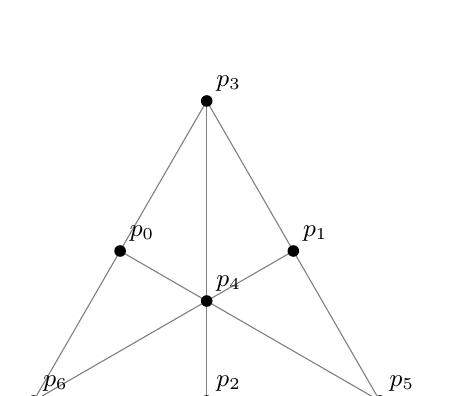
\begin{tikzpicture}[x=2.2cm,y=2.2cm,every node/.style={font=\small}]
  \coordinate (p0) at (0,0);
  \coordinate (p1) at (1,0);
  \coordinate (p2) at (0.5,-0.8660);
  \coordinate (p3) at (0.5,0.8660);
  \coordinate (p4) at (0.5,-0.2887);
  \coordinate (p5) at (1.5,-0.8660);
  \coordinate (p6) at (-0.5,-0.8660);
  \draw[gray] (p0)--(p3)--(p6);
  \draw[gray] (p0)--(p4)--(p5);
  \draw[gray] (p1)--(p3)--(p5);
  \draw[gray] (p1)--(p4)--(p6);
  \draw[gray] (p2)--(p3);
  \draw[gray] (p2)--(p5)--(p6);
  \foreach \i in {0,...,6}{\fill (p\i) circle (2.1pt) node[above right] {$p_\i$};}
\end{tikzpicture}
\caption{恰确定十一个圆的七点构造。灰色线段表示全部共线三元组；
未画出圆。}
\label{fig:c7}
\end{figure}
全部圆恰为
\[
0134,\ 0156,\ 0235,\ 0246,\ 1236,\ 1245,
012,\ 345,\ 346,\ 356,\ 456.
\]
前六个为四点圆，后五个为普通圆，故总数为十一。
程序
\file{computation/n4_to_8/n7/verify_extremal_configuration.py}
先对正定型 $x^2+xy+y^2$ 精确核验，再经显式欧氏变换
$(x,y)\mapsto(x+y/2,\sqrt3\,y/2)$ 用标准圆方程重新核验一次。

还可追问是否存在 $c(P)=12=F(7)-1$ 的中间构造；答案是否定的。若一条直线
或一个圆含至少五点，则引理~\ref{lem:largest} 已给出至少十三个圆。否则，令
$c_4$ 为四点圆数，令 $\ell=\ell_3+4\ell_4$，则
$c(P)=35-\ell-3c_4$，而点对计数给出 $\ell\le11$。恰有十二个圆只可能对应
\[
(c_4,\ell)=(4,11),(5,8),(6,5),(7,2).
\]
第一种情形没有普通直线，与 Sylvester--Gallai 定理矛盾
~\cite[pp.~111--112]{borwein-moser}；两个五圆族均不存在
相容的直线族。五个六圆关联轨道分别由引理~\ref{lem:two-line-geometry} 的两线
关系和四组精确坐标消元排除；其中一组会强迫原先缺少的第六条直线，从而回到上面的
十一圆构造。唯一的七圆轨道则由七点下界中保留一般正定二次型的计算排除。文件
\file{computation/n4_to_8/n7/classify_line_extensions.py}、
\file{verify_circle_count_spectrum.py} 与 \file{verify_q7_exclusion.py} 重现这些
有限分类和符号消元。因此不存在十二圆构造。

\subsection{\texorpdfstring{$c(8)=17<19=F(8)$}{c(8)=17<19=F(8)}}

先回顾 Elliott 所记录的 Segre 反例~\cite[p.~182, discussion following
Theorem~2]{elliott}。取两组同心、同向的正方形顶点
\[
(\pm1,\pm1),\qquad(\pm r,\pm r),\qquad r>0,\quad r\ne1.
\]
这是立方体沿一条面中心轴作中心投影后得到的关联结构。它有两条四点直线、
十个四点圆和八个三点圆。非共线三元组数为
\[
\binom83-2\binom43=48=10\binom43+8,
\]
故该构造确定 18 个圆。下面的有理坐标构造将圆数进一步降至 17。

取以下有理点：
\[
\begin{aligned}
p_0&=(0,0),\\
p_1&=\left(\frac{263}{626},\frac{2178}{4069}\right),&
p_2&=\left(\frac{263}{313},\frac{4356}{4069}\right),\\
p_3&=\left(\frac{789}{626},\frac{6534}{4069}\right),&
p_4&=\left(\frac{53519}{195938},\frac{1842342}{1273597}\right),\\
p_5&=\left(\frac{184032}{458545},\frac{7245468}{5961085}\right),&
p_6&=\left(\frac{160557}{917090},\frac{5527026}{5961085}\right),\\
p_7&=\left(-\frac{25}{313},\frac{312}{313}\right).
\end{aligned}
\]
\begin{figure}[ht]
\centering
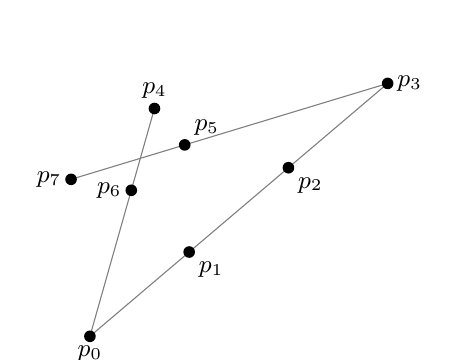
\begin{tikzpicture}[x=3.0cm,y=2.0cm,every node/.style={font=\small}]
  \coordinate (p0) at (0,0);
  \coordinate (p1) at (0.4201,0.5353);
  \coordinate (p2) at (0.8403,1.0705);
  \coordinate (p3) at (1.2604,1.6058);
  \coordinate (p4) at (0.2731,1.4465);
  \coordinate (p5) at (0.4013,1.2155);
  \coordinate (p6) at (0.1751,0.9272);
  \coordinate (p7) at (-0.0799,0.9968);
  \draw[gray] (p0)--(p3);
  \draw[gray] (p0)--(p4);
  \draw[gray] (p3)--(p7);
  \fill (p0) circle (2.1pt) node[below] {$p_0$};
  \fill (p1) circle (2.1pt) node[below right] {$p_1$};
  \fill (p2) circle (2.1pt) node[below right] {$p_2$};
  \fill (p3) circle (2.1pt) node[right] {$p_3$};
  \fill (p4) circle (2.1pt) node[above] {$p_4$};
  \fill (p5) circle (2.1pt) node[above right] {$p_5$};
  \fill (p6) circle (2.1pt) node[left] {$p_6$};
  \fill (p7) circle (2.1pt) node[left] {$p_7$};
\end{tikzpicture}
\caption{确定 17 个圆的有理八点构造。灰色线段表示全部极大共线子集；
全部圆在正文中列出。}
\label{fig:c8}
\end{figure}
其 17 个圆为
\begin{gather*}
0145,0167,024,0257,026,0347,0356,1247,1256,\\
1346,135,137,157,2345,2367,246,4567.
\end{gather*}
\file{computation/n4_to_8/n8/verify_construction.py} 只用有理数行列式核验这 17 个圆，并核验
全部 $\binom83=56$ 个三元组恰落在一个极大共线子集或一个所列圆中。对
至多 16 个圆的八点关联结构作同构分类后，没有任何一个通过实几何可实现性
检验，故 $c(8)\ge17$，从而 $c(8)=17$。

\subsection{例外构造的关联类型与 Möbius 模空间}
\label{sec:exceptional-moduli}

例外构造的关联类型与 Möbius 轨道是两个不同层次的概念：前者是有限组合数据，
后者还保留连续的交比参数。本文得到的完整关联分类如下。

\begin{proposition}\label{prop:exceptional-types}
在点重标号下，$(n,c(P))=(6,8),(7,11),(8,17)$ 各恰有一个可实现的直线--圆
关联类型。在 $(n,c(P))=(8,18)$ 层，抽象上共有十六个直线--圆关联类型，其中
恰有三个可在实平面中实现；它们的极大直线大小分别为 $(4,4),(4,3),(3,3)$。
忘记直线块与圆块的区别后，这三个类型合并为同一个广义圆关联类型。
上述四个可实现层中的每一个都含有连续统多个扩展 Möbius 轨道。
\end{proposition}

\begin{proof}
六点与七点的结论来自相应下界证明末端的同构分类。八点十七圆层共有七个抽象
直线--圆关联类型，精确的实可实现性排除后只留下极大直线为 $0123,046,357$ 的类型。
十八圆层由三元组唯一归属得到
\[
 \sum_L\binom{|L|}{3}
 +\sum_{C:\,|C|\ge4}\left(\binom{|C|}{3}-1\right)=38.
\]
在该恒等式下穷尽回溯得到十六个直线--圆关联类型。其中十二个类型属于同一个
广义圆关联类型；把其中一点送到无穷远点后会强迫 Fano 平面的实实现，故均不可能。
第二个广义圆关联类型强迫 Möbius--Kantor 关联方程，其最后一个行列式为
$-(t^2-t+1)$，判别式为 $-3$，同样不可能。余下的广义圆关联类型恰有命题所列
三种直线块与圆块的类别分配。文件
\file{computation/n4_to_8/orbit_classification/c17_exclusions/verify_target_records.py}
复核十七圆层的七个关联记录；同一目录中的精确证书逐一核验其实可实现性。文件
\file{computation/n4_to_8/orbit_classification/verify_incidence_types.py}
复核十八圆层的枚举、同构合并与两个不可实现证书。下列正维参数族及点重标号群的有限性
给出最后一个断言。
\end{proof}

为完整列明十八圆层的三个可实现直线--圆关联类型，下面各取一个代表；每项列出全部极大
直线与全部圆块，下标串采用第 2 节的约定，并以 $C_k$ 表示 $k$ 点圆块的列表。
\begin{itemize}
\item $(4,4)$ 型的直线为 $0145,2367$，且
\[
\begin{gathered}
C_3: 035,036,056,124,127,147,247,356,\\
C_4: 0123,0167,0246,0257,0347,1256,1346,1357,2345,4567.
\end{gathered}
\]
\item $(4,3)$ 型的直线为 $0145,036$，且
\[
\begin{gathered}
C_3: 035,056,124,127,147,247,356,\\
C_4: 0123,0167,0246,0257,0347,1256,1346,1357,2345,2367,4567.
\end{gathered}
\]
\item $(3,3)$ 型的直线为 $035,124$，且
\[
\begin{gathered}
C_3: 036,056,127,147,247,356,\\
C_4: 0123,0145,0167,0246,0257,0347,1256,1346,1357,2345,2367,4567.
\end{gathered}
\]
\end{itemize}

以下显式写出 Möbius 商。把 $\mathbb R^2$ 等同于 $\mathbb C$，并采用有序交比
\[
 [z_0,z_1;z_2,z_3]
 =\frac{(z_0-z_2)(z_1-z_3)}{(z_0-z_3)(z_1-z_2)}.
\]

\paragraph{六点八圆。}
选定下述关联标号并作相似变换归一化后，每个实现都唯一地表示为某个
\[
 (a,v)\in\mathcal U_6=
 \{(a,v)\in\mathbb R^2:a\ne0,1,\ v\ne0,\ a\ne1+v^2\}
\]
所对应的
\[
\begin{aligned}
p_0&=(0,0),&p_2&=(1,0),&p_4&=(a,0),&p_3&=(1,v),\\
s&=\frac{a}{1+v^2},&
t&=\frac{a(a-1)}{(a-1)^2+v^2},&
p_5&=(s,sv),&p_1&=(a+t(1-a),tv).
\end{aligned}
\]
其极大直线为 $024,035,134$，四点圆为 $0123,0145,2345$。令
\[
x=[p_0,p_1;p_2,p_3]
=\frac{a-1-v^2}{(a-1)(1+v^2)},\qquad
y=[p_0,p_1;p_4,p_5]
=\frac{a-1-v^2}{a-1}.
\]
则
\[
v^2=\frac{y-x}{x},\qquad a=\frac{y(1-x)}{x(1-y)}.
\]
未标号 Möbius 轨道空间为
\[
 \mathcal M_6=\mathcal D_6/\langle R,S\rangle,
 \qquad
 \mathcal D_6=\left\{(x,y):x,y\notin\{0,1\},\ \frac{y-x}{x}>0\right\},
\]
其中六阶群由
\[
 R(x,y)=\left(\frac1y,\frac1x\right),\qquad
 S(x,y)=\left(x,\frac{xy-2x+1}{y-x}\right)
\]
生成。每个构型还具有诱导置换
$(p_0p_1)(p_2p_3)(p_4p_5)$ 的 anti-Möbius 自同构，所以允许
anti-Möbius 变换不会进一步合并未标号六点轨道。

\paragraph{七点十一圆。}
选定下述关联标号后，每个实现也有唯一的相似归一化表示，对应于某个
\[
 (u,v)\in\mathcal U_7=
 \{(u,v)\in\mathbb R^2:u\ne0,1,\ v\ne0,\ u^2-u+v^2\ne0\}
\]
的形式。取
\[
 p_3=(0,0),\quad p_4=(1,0),\quad p_5=(u,v),\quad
 p_6=\left(u,\frac{u(1-u)}v\right),
\]
并令
\[
p_0=p_3p_6\cap p_4p_5,\qquad
p_1=p_3p_5\cap p_4p_6,\qquad
p_2=p_3p_4\cap p_5p_6.
\]
于是
\[
\begin{aligned}
p_0&=\left(\frac{v^2}{(u-1)^2+v^2},
           \frac{-v(u-1)}{(u-1)^2+v^2}\right),\\
p_1&=\left(\frac{u^2}{u^2+v^2},\frac{uv}{u^2+v^2}\right),
&p_2&=(u,0).
\end{aligned}
\]
其极大直线为 $036,045,135,146,234,256$，六个四点圆正是上文构造中列出的
前六个圆。$\mathcal U_7$ 上所有未标号保向 Möbius 等价由
\[
A(u,v)=\left(\frac{u}{u^2+v^2},\frac{-v}{u^2+v^2}\right),\qquad
B(u,v)=\left(\frac{v^2}{u^2-u+v^2},
             \frac{-v(u-1)}{u^2-u+v^2}\right)
\]
生成；所得群的阶为 $24$。故
\[
 \mathcal M_7^+=\mathcal U_7/\langle A,B\rangle,
 \qquad
 \mathcal M_7^{\pm}=\mathcal U_7/\langle A,B,C\rangle,
 \quad C(u,v)=(u,-v),
\]
而一般参数处的扩展群阶为 $48$。

\paragraph{八点。}
十七圆类型的极大直线为 $0123,046,357$。它包含如下有理一参数族：令
\[
m=\frac3{3-b^2},\qquad r=\frac{3(1+b^2)}{3-b^2},\qquad
t=\frac{b^2-3}{b^2+9},\qquad
O=\left(\frac{1-b^2}{1+b^2},\frac{2b}{1+b^2}\right),
\]
在反演前取
\[
\begin{aligned}
P_0&=(0,0),&P_1&=(1,0),&P_2&=(1,b),&P_6&=(r,0),\\
P_3&=(1+t(r-1),b(1-t)),&
P_4&=P_0P_3\cap P_1P_2,&P_5&=(m,mb).
\end{aligned}
\]
以 $O$ 为中心作半径平方为一的反演 $I_O$，并置
$p_i=I_O(P_i)$（$0\le i\le6$）、$p_7=O$。除去有限个代数退化参数后，所得构型
恰有上文十七圆构造的完整关联表。$b=13/12$ 给出上文坐标；$b=1$ 给出同一
直线--圆关联类型中另一个与它既不 Möbius 等价、也不 anti-Möbius 等价的构型。

十八圆层则含有一般的二参数位似矩形族
\[
 (\pm A,\pm1),\qquad(\pm rA,\pm r).
\]
该族实现含两条四点直线块的类型；在适当的广义圆交点处反演，可得到命题
~\ref{prop:exceptional-types} 中另外两种直线块与圆块的类别分配。参数恒等式与
非等价性检验分别见
\file{computation/n4_to_8/orbit_classification/verify_parametric_families.py} 和
\file{computation/n4_to_8/orbit_classification/verify_mobius_moduli.py}。

最后，若 $\lambda$ 是四个点的一种有序交比，则
\[
 J(\lambda)=\frac{(1-\lambda+\lambda^2)^3}
 {\lambda^2(1-\lambda)^2}
\]
与四点的次序无关，且在 Möbius 与 anti-Möbius 变换下不变。因此所有极大四点
广义圆的 $J$ 值多重集是未标号不变量。上述程序先比较该多重集，再对剩余的每个
关联重标号用精确的归一化交比判定。六点、七点公式给出完整 Möbius 模空间；八点
公式足以证明存在连续统多个轨道，但本文不声称所列一参数、二参数族已经穷尽相应
关联类型的全部实实现空间。

\section{无三点共线的加强版本}\label{sec:no-three}

下面证明推论~\ref{thm:no-three}。

\begin{proof}
先给出一般上界。在一个圆上取 $n-1$ 个点，再取一个避开这些点所确定的有限条
割线的圆外点。所得点集无三点共线，并且恰确定原来的大圆，以及圆外点和大圆上
每一对点所确定的一个不同圆。因此
$c_{\mathrm{nc}}(n)\le1+\binom{n-1}{2}$。

先证明 $n\ge11$ 时的反向不等式。由于每条直线至多含两点，此时 $K$ 就是一圆
所含点数的最大值。若 $3(K-1)<2(n-1)$，引理~\ref{lem:bojanowski-local} 的证明
可在 $b_i(x)=0$ 的条件下原样应用，得到
\[
\Phi_x\ge
\frac{K+1}{18K}\binom{n-1}{2}
+\frac{K+1}{2K}+\frac{(K-2)(n-1)}{9K}.
\]
对 $x$ 求和并减去 $1+\binom{n-1}{2}$ 后，所得余量为
\[
\frac{(n-4)\{Kn^2-13Kn+18K+n^2-7n\}}{36K}.
\]
该式关于 $K$ 单调递减；在 $K=(2n+1)/3$ 处等于
\[
\frac{(n-4)(n-1)(n^2-10n-9)}{18(2n+1)},
\]
对 $n\ge11$ 为正。

若 $3(K-1)\ge2(n-1)$，则最大圆外的一点绝不可能与最大圆上的一对点共线，
所以引理~\ref{lem:largest} 的圆情形加强为
\[
c(P)\ge1+(n-K)\binom K2-\binom{n-K}{2}
\left\lfloor\frac K2\right\rfloor
\ge1+\frac{(n-K)K(3K-n-1)}4.
\]
在 $(2n+1)/3\le K\le n-1$ 上，最后一个三次式的导函数为开口向下的二次式，
在左端为正、右端为负，故最小值出现在端点。两端相对于
$1+\binom{n-1}{2}$ 的余量分别为
\[
\frac{(n-4)(n-1)(2n-9)}{36}\qquad\hbox{和}\qquad0.
\]
这就证明了 $n\ge11$。

其余阶数可作较短处理。$n=4$ 时，若两个三元组属于同一个圆，则四点全共圆，
所以四个三元组给出四个不同圆。$n=5$ 时至多有一个四点圆，按圆分拆十个三元组
得到至少 $10-3=7$ 个圆。$n=6$ 时，若存在五点圆，上面的最大圆界给出十一；
否则每个非普通圆都含四点。两个四点圆至多交于两点，故它们在六点集中的补二元组
两两不交，于是四点圆至多有三个。三元组计数给出
$c(P)\ge20-3\cdot3=11$。

对 $n=7$，唯一可能低于目标值的情形由七个四点圆组成；在点重标号下，这些
四元组是 Fano 平面七条直线的补集。在一点处反演后，得到四条直线
$123,145,246,356$ 和三个圆 $1256,1346,2345$。归一化为
\[
p_1=(0,0),\quad p_2=(1,0),\quad p_3=(t,0),\quad
p_4=(u,v),\quad p_5=a(u,v),
\]
并令 $p_6=p_2p_4\cap p_3p_5$。约去已知非零的关联因子后，三个圆行列式为
\[
-a(u^2+v^2)+2tu-t,\qquad
a(u^2+v^2)-2au+t,\qquad
-a(u^2+v^2)+t.
\]
它们依次迫使 $u=1$、$v=0$、$a=t$，与所需的非共线性矛盾。因此
$c_{\mathrm{nc}}(7)=16$。点重标号下的有限分类由
\file{computation/no_three_collinear/verify_no_three_collinear.py} 重现。

对 $n=9$，若每个圆至多含四点，并以 $c_4$ 表示四点圆数，则
$c(P)=\binom93-3c_4$。固定一点，经过该点的四点圆在其余八点上给出若干三元组，
任意点对至多出现一次，故这类三元组至多有
$\lfloor(8/3)\lfloor7/2\rfloor\rfloor=8$ 个。对九个点求和并除以四，得到
\[
c_4\le\left\lfloor\frac94
\left\lfloor\frac83\left\lfloor\frac72\right\rfloor\right\rfloor
\right\rfloor=18
\]
个，故 $c(P)\ge30$。若存在至少五点的圆，则由加强后的最大圆界得到所需下界
$29$。

对 $n=10$，同一最大圆界处理 $K\ge6$。若 $K\le5$，在 $x$ 处反演，并以
$(t_2,t_3,t_4)$ 表示九个像点的连接线重数。点对计数、Melchior 不等式和
Hirzebruch 不等式给出
\[
t_2+3t_3+6t_4=36,\qquad t_2\ge3+t_4,\qquad t_2\ge2t_4.
\]
又有 $t_2\equiv0\pmod3$。对 $0\le t_4\le4$ 直接代入可得
\[
\frac{t_2}{3}+\frac{t_3}{4}+\frac{t_4}{5}\ge\frac{18}{5},
\]
且等号只在 $(t_2,t_3,t_4)=(6,4,3)$ 成立。若 $c(P)\le36$，则十个反演中心
处均须取等号。于是应有六个五点圆，每点恰在其中三个圆上，且任意两个圆恰交于
两个点；所得 $2$-$(6,3,2)$ 关联设计在重标号下只有一个轨道。这一有限断言由
\file{computation/no_three_collinear/verify_no_three_collinear.py} 从全部带标号三元组
精确枚举得到。

在属于其中第 $0,1,4$ 个块的一点处反演。其余九点各四点一组地落在一个三角形的
三条边上。作仿射归一化，把每条边上的另两点写成
\[
(u,0),(v,0),\qquad(0,s),(0,t),\qquad(p,1-p),(r,1-r),
\]
同时保留一般正定二次项 $x^2+2kxy+hy^2$。前两个五点圆方程给出
$hs=uv$ 与 $hst=u$，从而 $t=1/v$、$h=uv/s$。从其余方程中消去 $k$ 后得到
\[
p(s+1)=1,\qquad r(u+1)=u,\qquad(v-1)(su-1)=0.
\]
点互异给出 $v\ne1$，故 $su=1$，进而 $p=r$，再次出现重合点。因此
$c_{\mathrm{nc}}(10)=37$。

最后处理例外阶数八。由两个同心正方形
$(\pm1,\pm1),(\pm2,\pm2)$ 出发；该点集确定十八个圆和两条极大直线。以
$z=(0,10)$ 为中心作反演。点 $z$ 不在这二十个广义圆中的任何一个上，故它们
全部变成圆，且像点集无三点共线。像点的有理坐标为
\[
\begin{gathered}
(1/82,811/82),(1/122,1209/122),(-1/82,811/82),(-1/122,1209/122),\\
(1/34,168/17),(1/74,367/37),(-1/34,168/17),(-1/74,367/37).
\end{gathered}
\]
图~\ref{fig:no-three-eight} 是上述精确坐标经平移和等比例放大后的点图。按照
第 2 节的下标串约定，其二十个圆为
\begin{gather*}
0123,0145,0167,0246,0257,0347,035,036,056,124,\\
1256,127,1346,1357,147,2345,2367,247,356,4567.
\end{gather*}
\begin{figure}[ht]
\centering
\begin{tikzpicture}[scale=0.82,every node/.style={font=\small}]
  \coordinate (p0) at (1.2195,1.0244);
  \coordinate (p1) at (0.8197,2.9836);
  \coordinate (p2) at (-1.2195,1.0244);
  \coordinate (p3) at (-0.8197,2.9836);
  \coordinate (p4) at (2.9412,0.2353);
  \coordinate (p5) at (1.3514,3.8919);
  \coordinate (p6) at (-2.9412,0.2353);
  \coordinate (p7) at (-1.3514,3.8919);
  \fill (p0) circle (2.2pt) node[right] {$p_0$};
  \fill (p1) circle (2.2pt) node[right] {$p_1$};
  \fill (p2) circle (2.2pt) node[left] {$p_2$};
  \fill (p3) circle (2.2pt) node[left] {$p_3$};
  \fill (p4) circle (2.2pt) node[right] {$p_4$};
  \fill (p5) circle (2.2pt) node[above right] {$p_5$};
  \fill (p6) circle (2.2pt) node[left] {$p_6$};
  \fill (p7) circle (2.2pt) node[above left] {$p_7$};
\end{tikzpicture}
\caption{无三点共线加强版本中的八点构造。这里只画出点；若同时画出全部
二十个圆，图形反而难以辨认。}
\label{fig:no-three-eight}
\end{figure}
所以 $c_{\mathrm{nc}}(8)\le20$。

为证下界，最大圆界先排除至少含五点的圆。若所有圆至多含四点，则
$c(P)=56-3c_4$。定理~\ref{thm:main} 已给出 $c(P)\ge17$，因而低于二十的
唯一可能值是十七。对四元组的精确分类表明，在无三点共线的条件下，十七圆层
只有一个关联类。反演并重标号后，它给出六条直线
\[
036,045,135,146,234,256
\]
以及七个所需圆
\[
0134,0156,0235,0246,1236,1245,3456.
\]
令 $p_0=(0,0)$、$p_1=(1,0)$、$p_3=(0,1)$，并写
$p_6=(0,a)$、$p_5=(b,1-b)$；其余点由直线关联唯一确定。对一般二次项
$x^2+2kxy+hy^2$，前两个圆条件给出
\[
h=-\frac{b}{a-b+1},\qquad k=\frac{1-b}{a-b+1}.
\]
代入后，圆 $3456$ 的行列式分子为
\[
2ab^2(a-1)^2(b-1)(ab-b+1).
\]
点互异、已列直线关联和二次型正定性保证每个因子都非零，矛盾。因此十七圆
关联类不能由无三点共线的欧氏点集实现，故 $c_{\mathrm{nc}}(8)=20$，证明完成。
\end{proof}

\begin{remark}
文件 \file{computation/no_three_collinear/verify_no_three_collinear.py} 独立核验上述证明中
的全部有限分类与多项式恒等式，以及八点有理构造。所有判断均使用精确整数、有理数
或符号多项式运算，不以数值近似根作为证据。
\end{remark}


\appendix
\section{早期的 \texorpdfstring{$n\ge92$}{n>=92} 证明}
\label{app:early92}

本节记录最初从 Eureka 数值结果中提炼出的中间论证。正文中 $n\ge17$ 的证明已经
在逻辑上取代了它；这里保留这一证明，是为了说明数值阈值如何先被转化为简短的
数学论证，随后再继续加强。

\begin{proposition}
若 $n\ge92$，则每个合格 $n$ 点集都至少确定 $F(n)$ 个圆。
\end{proposition}

\begin{proof}
令 $K$ 为最大直线块或最大圆块的大小，并置 $r=n-K$。按照 $K$ 是否至少为
$3n/8$ 分成两种情形。

先设 $K\ge3n/8$。引理~\ref{lem:largest} 中的两个量满足
\[
 D_L(n,r)-D_C(n,r)=r\left\lfloor\frac K2\right\rfloor-1\ge0.
\]
再在圆块下界中使用 $\lfloor K/2\rfloor\le K/2$，则无论最大块是直线还是圆，均有
\begin{equation}\label{eq:early-B}
 c(P)\ge B(n,K):=1+\frac{(n-K)K(3K-n-3)}4.
\end{equation}
当 $K=n-1$ 时，精确下界 $D_C(n,1)$ 就是 $F(n)$。以下可设
$3n/8\le K\le n-2$。在该区间上
\[
 \frac{\partial^2 B}{\partial K^2}
 =\frac{-18K+6n+6}{4}<0,
\]
故 $\partial B/\partial K$ 严格递减，$B$ 不会在区间内部取得最小值，只需考察两个
端点。注意
\begin{equation}\label{eq:early-F-upper}
 F(n)\le1+\frac{(n-2)^2}{2}.
\end{equation}
两个端点相对于该上界的余量分别为
\[
 B\left(n,\frac{3n}{8}\right)-1-\frac{(n-2)^2}{2}
 =\frac{15n^3-1384n^2+4096n-4096}{2048}
\]
和
\[
 B(n,n-2)-1-\frac{(n-2)^2}{2}
 =\frac{(n-2)(n-7)}2.
\]
在第一式中令 $n=92+u$，其分子化为
\[
15u^3+2756u^2+130320u+338880,
\]
第二个余量也显然为正，因此第一种情形成立。

以下设 $K<3n/8$。固定反演中心 $x\in P$，并置 $N=n-1$、$M=K-1$。反演像中的
每条连接线至多含 $M$ 个像点。若 $t_i$ 表示其中恰含 $i$ 个像点的连接线数，定义
\[
 a_M=
 \begin{cases}
 6,&2\le M\le9,\\[2pt]
 \displaystyle\frac{\binom M2}{M-3},&M\ge10,
 \end{cases}
 \qquad
 y_M=\frac1{a_M+1},\qquad z_M=1-y_M.
\]
由 $a_M$ 的定义，
\[
 y_M\binom i2\le z_M(i-3)\qquad(4\le i\le M).
\]
把点对恒等式与 Melchior 不等式按第 2 节的方法线性组合，得到
\begin{equation}\label{eq:early-dual}
 t_2+t_3\ge y_M\binom N2+3z_M
 =3+y_M\left(\binom N2-3\right).
\end{equation}
其中至多 $\lfloor N/2\rfloor$ 条二点线或三点线经过反演中心。其余每条线反演为
一个经过中心、总共含三个或四个原点的圆；对全部中心求和后，每个这样的圆至多
被计数四次。因此
\begin{equation}\label{eq:early-inversion}
 c(P)\ge\frac n4\left[
 3+y_M\left(\binom{n-1}{2}-3\right)
 -\left\lfloor\frac{n-1}{2}\right\rfloor\right].
\end{equation}

由于 $K<3n/8$ 且 $K$ 为整数，
\[
 M=K-1\le\frac{3n-9}{8}=:M_0.
\]
函数
\[
 g(s)=\frac{2(s-3)}{(s+3)(s-2)}
\]
在 $s\ge6$ 时递减。对 $M\ge10$ 有 $y_M=g(M)$，对 $M\le9$ 则有
$y_M=1/7=g(9)$，故
\[
 y_M\ge g(M_0)=\frac{16(n-11)}{(n+5)(3n-25)}.
\]
在式~\eqref{eq:early-inversion} 中以 $(n-1)/2$ 代替取整项，再使用
式~\eqref{eq:early-F-upper}，所得下界减去 $F(n)$ 至少为
\[
 \frac{n^4-105n^3+787n^2-1931n+3000}
 {8(n+5)(3n-25)}.
\]
令 $n=98+u$，分子变为
\[
 u^4+287u^3+27541u^2+891829u+783766,
\]
故对所有 $n\ge98$ 均为正。

只剩 $92\le n\le97$。下表中，$K_0$ 是严格小于 $3n/8$ 的最大整数，
$M_0=K_0-1$，而 $\Delta_n$ 是在 $M_0$ 处计算的式~\eqref{eq:early-inversion}
右端减去 $F(n)$。式~\eqref{eq:early-dual} 的下界随 $M$ 增大而减小，故表中列出的
正是第二种情形的最小余量。
\[
\begin{array}{c|rrrrrr}
n&92&93&94&95&96&97\\ \hline
K_0&34&34&35&35&35&36\\
M_0&33&33&34&34&34&35\\
\Delta_n&43&88&\frac{20371}{1184}&\frac{9225}{148}&
\frac{4908}{37}&\frac{29823}{836}
\end{array}
\]
六个余量均为正，证明完成。
\end{proof}

\begin{remark}
上述论证没有枚举任何关联结构；表格只核验六条精确有理数端点不等式。正文证明把
这一早期阈值推进到 $n\ge17$，后续两节再分别处理 $n=16$ 与 $n=15$。
\end{remark}

\section{精确验证与独立复现}\label{app:verification}

经审计的材料由两个相互独立的入口复现。先在 \file{Erdos506} 目录运行
\begin{center}
\file{computation/verify_certified_results.py}
\end{center}
\begin{verbatim}
python computation/verify_certified_results.py
\end{verbatim}
该命令重检 $n\ge15$ 的数学恒等式、$n\le8$ 的精确构造与分类，以及
推论~\ref{thm:no-three}。中间六层另由
\begin{verbatim}
cd computation/n9_to_14
python run_verification.py --jobs 8 --seconds 240
\end{verbatim}
完整复现，细节见下文。两个入口都不把随机搜索、浮点可行性、超时或未知求解
状态用作排除证书。二者均要求 CPython~3.13，以匹配经审计的二进制模块；SymPy 用于精确多项式运算，项目固定
使用 OR-Tools 9.15.6755，且只通过
\file{computation/runtime_dependencies.py} 加载并核验版本。

\subsection{数学证明范围}

\begin{longtable}{P{6.4cm}P{8.1cm}}
\toprule 文件 & 独立核验内容\\ \midrule
\file{computation/n_ge_17/verify_n_ge_17.py} &
用有理数展开引理~\ref{lem:bojanowski-local} 的系数差、两个奇偶多项式、
端点余量及最大块代数\\
\file{computation/n16/verify_n16.py} &
展开 $K=7,8$ 的两条恒等式，核对全部非负余项、唯一等号型、圆相交二阶矩
以及 $K=9,\ldots,15$ 的直接界\\
\file{computation/n9_to_14/verify_largest_block_reduction.py} &
核对十五点情形全部 $K\ge8$ 最大块的直线界与圆界\\
\file{computation/n15/verify_n15.py} &
核对 Cuntz 十四线表中的局部余量、正亏量估计、
式~\eqref{eq:n15-global-identity} 的全部系数及最后的同余矛盾；同时核对所引
记录用于识别所引参考文献 PDF 的 SHA-256 摘要\\
\bottomrule
\end{longtable}
这些脚本只核验正文已经给出的数学证明。十五点核验只读取正文列出的三个已发表
重数向量，不选择带标号点子集，也不枚举几何轨道或坐标。

$n\ge15$ 证明所用的算术与有限求和推论还形式化于
\begin{center}
\file{lean/Erdos506Nge15.lean}。
\end{center}
该文件使用项目固定的 Lean~4 与 Mathlib 工具链编译，不含 \texttt{sorry}、
\texttt{admit}、自定义公理声明或不安全定义。其形式化边界是明确的：正文引用的
欧氏与实射影关联定理在相应 Lean 定理中作为假设输入，而从这些假设推出的全部
代数结论均由内核检查。因此，它形式化的是证明的算术--组合部分，而不是底层
射影几何本身的形式构造。

推论~\ref{thm:no-three} 的算术--组合部分相应形式化于
\begin{center}
\file{lean/Erdos506NoThreeCollinear.lean}。
\end{center}
该文件由 Lean 内核检查六点、九点 packing 推导，十点局部等号情形，大阶证明的
两个端点因子，八点模三间隙，以及所有 $n\ge4$ 的最终分类讨论。随附的
\file{lean/compile_audit_no_three_collinear.json} 记录了 Lean~4.29.1 与 Mathlib 提交
\texttt{5e932f97} 下把警告视为错误的成功编译；源码不含证明占位符或新增公理。
与上文相同，欧氏关联引理和穷尽有限分类的输出均作为显式假设输入。

\subsection{九点至十四点}

这六层的源码位于
\begin{center}
\file{computation/n9_to_14/}。
\end{center}
在该目录运行
\begin{verbatim}
python run_verification.py --jobs 8 --seconds 240
\end{verbatim}
即可完整重放。工作进程数可以改变而不改变模型。每个求解器使用固定随机种子；超时记为
\texttt{UNKNOWN} 并继续保留。成功重放最终生成
\file{certificates/manifest.json}，其中七项终止检查均为真，总状态为
\texttt{PASS}。若重放在所有终止证书写出后被中断，可用
\file{audit_manifest.py} 重新进行同一终止状态及 SHA-256 审计。
当前下界表使用 $c(7)=11$；本包中的全部证书均在这一修正后重新生成。特别地，
十二点递归现在产生 622 个九点子计数向量，而不是旧版的 617 个。

各文件按数学作用分类如下。
部分文件名保留了实现阶段的英文术语：其中 \texttt{signature} 指第
~\ref{sec:small-uniform} 节定义的全局计数向量，\texttt{profile} 指附着于
点对的次数数据，\texttt{support} 指实际选取的带标号点子集；它们不是额外的
数学概念。
\begin{longtable}{P{6.2cm}P{8.3cm}}
\toprule 文件 & 在验证中的作用\\ \midrule
\file{signature_filters.py} & 由
\eqref{eq:small-line-pairs}--\eqref{eq:small-triple-partition}、最大块界、删除平均及文中引用的直线排列不等式生成全部全局计数向量\\
\file{projected_arrangement_model.py} & 生成全部局部重数向量及其直线/圆分拆；最终源码不包含历史的单线删除障碍表\\
\file{verify_local_type_filter.py} & 检查局部重数向量的精确无标号求和，并写出
\file{nN_01_signature_filter.json}\\
\file{verify_augmented_line_melchior.py} & 先检查
\eqref{eq:augmented-line-summed}，再检查所有点处的数据总和是否满足
\eqref{eq:augmented-line-point}；写出 02、03 号证书\\
\file{filter_by_classified_split_endpoints.py} & 检查
\eqref{eq:small-category-totals}--\eqref{eq:small-pair-profile2} 中连接点次数与点对次数的一致性恒等式；入口明确关闭两个可选有限目录\\
\file{pair_profile_generator.py},
\file{verify_pair_moment_filter.py} & 生成全部点对次数数据，并加入交集大小之和、交集大小二阶二项式系数之和及不交三点组计数；写出 05 号证书\\
\file{block_intersection_rows.py},
\file{block_row_existence_filter.py} & 在 $n=10$ 时，对每个出现的块加入三层精确三点组恒等式及两个块之间的匹配数上界，把 21 个计数向量降为 12 个\\
\file{verify_recursive_inversion_rows.py} & 把每个局部重数向量映射为低一阶完整计数向量，逐层平衡各点处的数据，并在九点基例中把极大直线和圆选为带标号点的子集\\
\file{verify_n10_final_radical_axis.py} & 重新生成两个匹配轨道、唯一剩余的直线设计轨道及排除最后十点计数向量的五个精确子式；程序先读取 07 号证书、记录其 SHA-256 摘要，并检查所保留的局部向量确实强制两个五点圆分割点集\\
\file{verify_n13_n14_global_inequalities.py} & 独立生成 3962 与 8981 个原始计数向量，并检查全局排除及
\eqref{eq:n13-global-two-ineq}；不选择任何带标号点子集\\
\file{run_verification.py}, \file{audit_manifest.py} & 按顺序执行各阶段，并检查所有终止状态、唯一的十点中间计数向量、文件大小和 SHA-256 摘要\\
\bottomrule
\end{longtable}

终止证书为
{\raggedright
\begin{description}[style=nextline,leftmargin=2.8em]
\item[$n=9$] \file{certificates/n9_04_exact_support.json}。
\item[$n=10$] \file{certificates/n10_07_recursive.json} 与
  \file{certificates/n10_08_final_geometry.json}。
\item[$n=11$] \file{certificates/n11_06_recursive.json}。
\item[$n=12$] \file{certificates/n12_06_recursive.json}。
\item[$n=13,14$] \file{certificates/n13_n14_global_inequalities.json}。
\end{description}
\par}
中间文件名带有表中所示的数字前缀，并严格按此前缀顺序读取。凡阶段读取上游证书，均记录其路径与 SHA-256 摘要。最终清单记录四十二个源码与证书文件。因此读者可以删除
\file{certificates} 目录，再由所列源码完整生成验证链。

本次四进程审计重放的总墙钟时间为 348.52 秒。最大的带标号基例模型含 840 个
布尔变量和 546 条约束；最慢的单个递归求解用时 6.62 秒，没有任何求解接近
240 秒上限。这些数据只用于说明规模，不是证书所依赖的假设。

复现应使用 CPython~3.13，因为经审计的二进制模块是对应的 CPython~3.13 构建。
整数求解器固定为 OR-Tools 9.15.6755，并仅通过
\file{computation/runtime_dependencies.py} 加载。SymPy 只用于十点末例的精确多项式运算。浮点可行性、随机搜索以及不是明确不可行的求解状态，均不用于排除任何情形。


\subsection{六点与七点}

\file{computation/n4_to_8/n6/verify_construction.py} 在 $\mathbb Q(\sqrt3)$ 中精确核验
六点坐标、极大直线、圆方程和三元组归属；
\file{computation/n4_to_8/n6/verify_lower_bound.py} 重现六点下界最后
一个有限参数情形。

七点的独立复现顺序如下：
\begin{enumerate}
\item \file{computation/n4_to_8/n7/classify_quad_packings.py}
分类至少五个四点圆组成的圆族，得到两个五圆类及各一个六圆、七圆类；
\item \file{computation/n4_to_8/n7/classify_line_extensions.py}
证明只有六圆族、七圆族可能满足 $c(P)\le10$；它同时核验唯一六圆候选没有
普通直线，并核验每个七圆候选都含正文使用的同一个两直线核心；
\item \file{computation/n4_to_8/n7/verify_q7_exclusion.py}
核验正文中的正定二次型约化；\file{verify_extremal_configuration.py}
则用精确欧氏圆方程核验十一圆构造。
\item \file{verify_circle_count_spectrum.py} 在十一圆和十二圆两层重新运行
关联分类，并核验四组符号约化，从而核对十一圆层并证明十二圆构造不存在。
\end{enumerate}
正定二次型脚本断言正文所用的两个有理因式分解，并记录全部非零分母；它不作
近似求根，也不扫描坐标。该表述在仿射归一化下保持正确；旧版只保留标准圆方程、
遗漏交叉项与第二个对角系数的归一化不再使用。
第三步所有文件均位于
\file{computation/n4_to_8/n7/}。

\subsection{八点}

以下文件除特别说明外均位于
\file{computation/n4_to_8/n8/}。
\begin{enumerate}
\item 首先由引理~\ref{lem:largest} 排除所有至少含五点的直线或圆；该步由
\file{computation/n9_to_14/verify_largest_block_reduction.py}
核验。正文的计数论证先排除十二圆以下的全部层；
\file{classify_boundary_layers.py} 随后为圆数 $12,\ldots,16$ 统一建立两个
穷尽分支：在点重标号下固定一条四点直线，或假设不存在四点直线。除三元组归属
与相交上界外，模型只再使用果园上界 $\ell_3\le7$、恒等式
$\ell_2=28-3\ell_3-6\ell_4$，以及 Melchior 不等式
$\ell_2\ge3+\ell_4$。
对全部点重标号轨道加入阻断子句后即得到穷尽分类。证书
\file{boundary_layer_classification.json} 记录十二至十六圆时的类别数依次为
$1,1,1,3,3$。
\item 几何排除独立于组合求解器。
\file{pattern1_inversion_relation.py}、\file{pattern1_inversion_circles.py}
核验十五圆特殊类的反演方程；
\file{no_four_line_inversion_relations.py}、\file{no_four_line_key_equations.py}
核验十六圆特殊类的消元方程。其余类别由引理~\ref{lem:two-line-geometry}
中的根轴断言排除。
对十五圆的特殊类，在两条规定直线的交点处反演，取两线为坐标轴，使
$0,1,2=(x_0,0),(x_1,0),(x_2,0)$、$4,5=(0,y_4),(0,y_5)$；欧氏二次型为
$x^2+y^2+2kxy$，其中 $k^2\ne1$。两脚本核验的共线式及第一个圆方程给出
\[
R=x_0x_1-2x_0x_2+x_1x_2=0,\qquad x_0x_2=y_4y_5.
\]
若 $x_0x_2=y_4^2$，则 $y_4=y_5$，故该因子非零。再令
$A=x_0x_2+y_4^2$、$B=y_4(x_0+x_2)$，后两个圆方程化为
$A=kB$ 与 $kA=B$。于是 $A=B=0$，从而 $x_0+x_2=0$；代回 $R=0$
得到 $2x_0^2=0$，与点互异矛盾。这就是该符号输出在此类别中使用的完整
几何推论。
\item \file{computation/n4_to_8/n8/verify_construction.py} 最后用精确有理行列式核验
十七圆构造，并检查全部 $56$ 个三元组的唯一归属。
\end{enumerate}

\subsection{例外关联类型与 Möbius 参数}

本段所有路径均位于
\file{computation/n4_to_8/orbit_classification/}。依次运行
\begin{center}
\begin{tabular}{l}
\file{python}\ \file{verify_incidence_types.py}\\
\file{python}\ \file{verify_parametric_families.py}\\
\file{python}\ \file{verify_mobius_moduli.py}\\
\file{python}\ \file{family_examples.py}
\end{tabular}
\end{center}
分别核验十八圆层的关联分类、正文各参数族的直线与圆恒等式、六点和七点的完整
有限商作用，以及所选参数族成员间的严格不等价性。子目录
\file{c17_exclusions/} 包含十七圆层的七个关联记录、唯一可实现类型的有理坐标
核验，以及对其余六类的符号消元或 Gröbner 基排除。\file{README.md} 给出完整
重现顺序，并区分“从头生成分类记录”与“核验已发布记录”这两项操作。

\subsection{无三点共线的加强版本}

单个文件 \file{computation/no_three_collinear/verify_no_three_collinear.py} 独立核验
推论~\ref{thm:no-three} 中的全部有限与代数断言。它统计反演后的双正方形构造
恰有二十个圆，展开大 $n$ 证明的两个端点余量，枚举七点、八点证明中唯一的
四元组 packing，分类十点等号分支中的 $2$-$(6,3,2)$ 设计，并核验各坐标消元式。
有限枚举从全部带标号子集出发，再与点集全置换所得轨道比较；坐标运算则完全在
有理数域或符号多项式环中进行。

\begin{remark}[从原始约束重放]
分类器从全部有标号三元组、四元组和五元组重新建立约束；JSON 文件是输出而
不是公理。轨道阻断逐一作用所有点置换。因此读者可删除生成的 JSON 后重新运行。
在同构完备性步骤中固定使用单工作线程。只有显式状态 \texttt{INFEASIBLE} 才排除
候选；其他状态一律保留候选，且任何非终止状态都会使相应证书标为不完整。
\end{remark}

\begin{thebibliography}{99}
\small
\bibitem{balintova}
A.~B\'alintov\'a and V.~B\'alint,
\emph{On the number of circles determined by $n$ points in the Euclidean plane},
Acta Math. Hungar. \textbf{63} (1994), 283--289.

\bibitem{burr-grunbaum-sloane}
S.~A.~Burr, B.~Grünbaum and N.~J.~A.~Sloane,
\emph{The orchard problem},
Geom. Dedicata \textbf{2} (1974), 397--424.

\bibitem{borwein-moser}
P.~Borwein and W.~O.~J.~Moser,
\emph{A survey of Sylvester's problem and its generalizations},
Aequationes Math. \textbf{40} (1990), 111--135,
doi:10.1007/BF02112289.

\bibitem{csima-sawyer}
J.~Csima and E.~T.~Sawyer,
\emph{There exist $6n/13$ ordinary points},
Discrete Comput. Geom. \textbf{9} (1993), 187--202.

\bibitem{cuntz}
M.~Cuntz,
\emph{Simplicial arrangements with up to 27 lines},
Discrete Comput. Geom. \textbf{48} (2012), 682--701.

\bibitem{elliott}
P.~D.~T.~A.~Elliott,
\emph{On the number of circles determined by $n$ points},
Acta Math. Acad. Sci. Hungar. \textbf{18} (1967), 181--188.

\bibitem{hirzebruch}
F.~Hirzebruch,
\emph{Singularities of algebraic surfaces and characteristic numbers},
Contemp. Math. \textbf{58} (1986), 141--155.

\bibitem{lin-et-al}
A.~Lin, M.~Makhul, H.~Nassajian Mojarrad, J.~Schicho,
K.~Swanepoel and F.~de Zeeuw,
\emph{On sets defining few ordinary circles},
Discrete Comput. Geom. \textbf{59} (2018), 59--87.

\bibitem{purdy-smith}
G.~B.~Purdy and J.~W.~Smith,
\emph{Lines, circles, planes and spheres},
Discrete Comput. Geom. \textbf{44} (2010), 860--882,
doi:10.1007/s00454-010-9270-3.

\bibitem{pokora}
P.~Pokora,
\emph{Extremal properties of line arrangements in the complex projective plane},
in \emph{Analytic and Algebraic Geometry 3}, L\'od\'z University Press, 2019,
191--200, doi:10.18778/8142-814-9.14.

\bibitem{shnurnikov}
I.~N.~Shnurnikov,
\emph{A $(t_k)$ inequality for arrangements of pseudolines},
Discrete Comput. Geom. \textbf{55} (2016), 284--295.

\bibitem{zhang}
R.~Zhang,
\emph{On the number of ordinary circles determined by $n$ points},
Discrete Comput. Geom. \textbf{46} (2011), 205--211.
\end{thebibliography}

\end{document}
